\section{Explanation for large charges based on secondary electron emission}\label{sec:see}

\subsection{The structure of MCP-PMT}\label{subsec:structure}
MCP-PMT deploies two pieces of MCPs as the electron multiplier.
The photoelectrons are amplified by MCP through a branching process described in Sec.~\ref{gammapossion}
and a large number of electrons produced at the end of the MCP reach the anode to form electrical signals~\cite{2013Photodetectors}.

\begin{figure}[H]
    \centering
    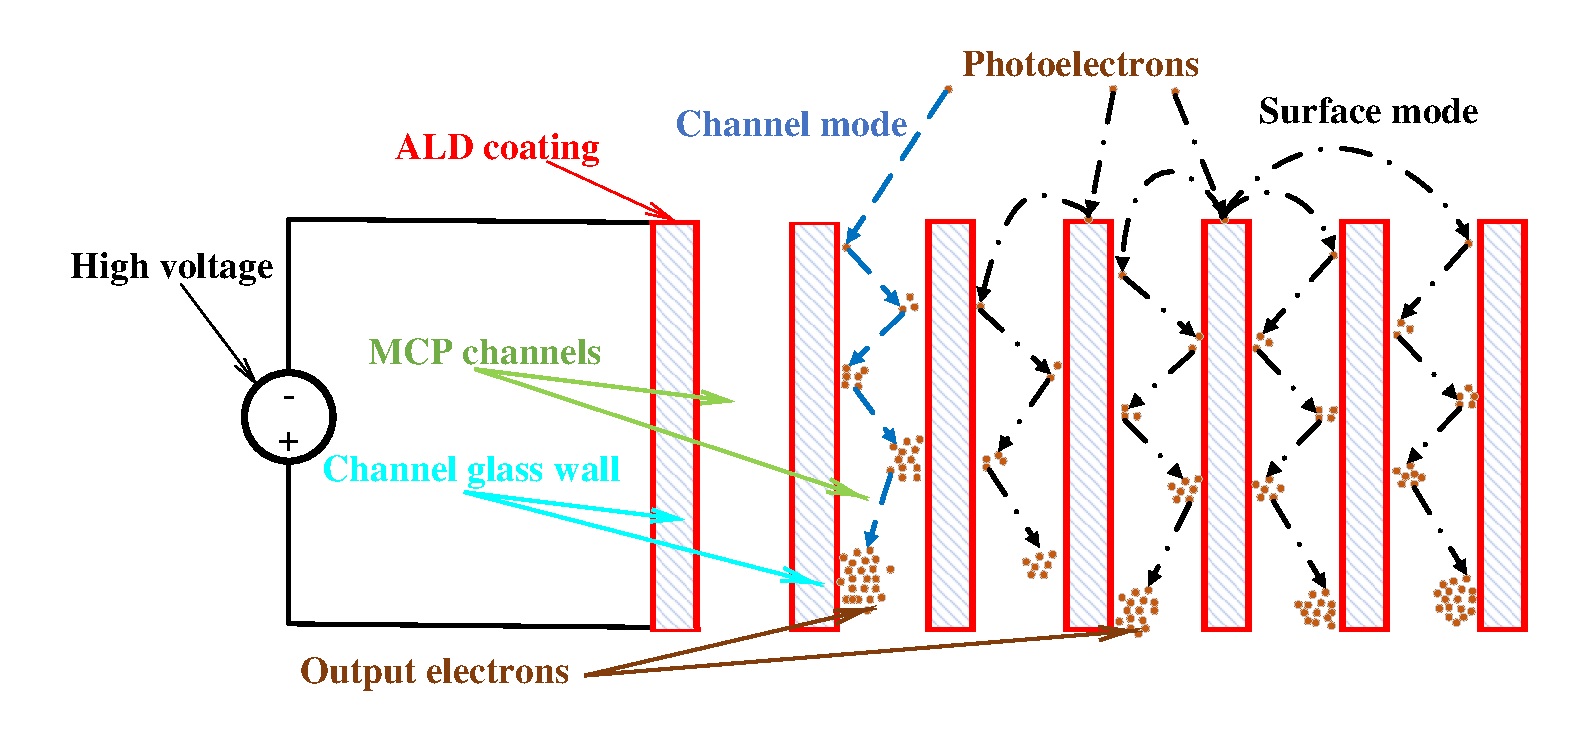
\includegraphics[width=0.7\textwidth]{pic/mcp.pdf}
    \caption{The photoelectrons directly enter the channels~(channel mode) or hit the upper surface producing secondary electrons
        which enter the channels later~(surface mode)~\cite{2016Optimization}. After entering the MCP channel, the electron collides
        with the channel wall for many times and is amplified in a series of such multiplications~\cite{1955Scintillation}.}\label{fig:MCP}
    \label{fig:mcp_modes}
\end{figure}

Besides, the secondary electrons from the upper surface of MCP can also enter the MCP channels for multiplication
under the influence of electric field.\@
Two independent mode dominate the amplification process as shown in Fig.~\ref{fig:mcp_modes}.
The \textit{channel mode} is that photoelectrons directly enter the channels
and the other is the \textit{surface mode} that secondary electrons from the upper surface enter the channels.
The selection of these two modes follows Bernoulli distribution~\cite{1955Scintillation}.

\subsection{Furman probabilistic model}\label{subsec:fuman}
The Furman probabilistic model~(Furman model)~\cite{2002Probabilistic}
is a theoretical framework employed to elucidate the phenomenon of SEE from solid surfaces.
This model incorporates the statistical nature of the SEE process
by considering the probability distribution governing the number of secondary electrons emitted per incident primary electron.
Each emission event of a secondary electron is regarded as an independent occurrence,
with its energy following the distribution contingent upon material properties and the primary energy.

In Furman model, the SES can be represented as $d\delta/dE$,
where $E$ is the energy of secondary electron.
There are three kinds of secondary electrons emitted.
The first kind is the back-scattered electron that secondary electrons are emitted by elastic scattering on the surface of the target material.
The SES is defined as Eq.~\eqref{eq:backscatter},
where $\delta_{\mathrm{bs}}$ is the yield of back-scatter electron,
$\theta(E)$ function ensures the $E<E_0$,
$E_0$ is the incident energy of the primary electron,
$\theta_0$ is the incident angle,
and $\sigma_{\mathrm{bs}}$ is an adjustable standard deviation.
\begin{equation}
    \label{eq:backscatter}
    \begin{aligned}
         & \frac{\delta_{\mathrm{bs}}}{dE} =\theta(E) \theta\left(E_0-E\right) \delta_{\mathrm{bs}}\left(E_0, \theta_0\right)
        \frac{2 \exp \left(-\left(E-E_0\right)^2 / 2 \sigma_{\mathrm{bs}}^2\right)}{\sqrt{2 \pi} \sigma_{\mathrm{bs}}
        \operatorname{erf}\left(E_0 / \sqrt{2} \sigma_{\mathrm{bs}}\right)}                                                   \\
    \end{aligned}
\end{equation}

The second kind is the rediffused electron that secondary electrons are generated by atomic scattering after electrons enter the target material.
The SES of rediffused electrons is defined as Eq.~\eqref{eq:rediffused},
where $\delta_{\mathrm{rd}}$ the yield of rediffused electron,
and $q$ is an adjustable parameter.
\begin{equation}
    \label{eq:rediffused}
    \begin{aligned}
         & \frac{\delta_{\mathrm{rd}}}{dE} =\theta(E) \theta\left(E_0-E\right) \delta_{\mathrm{rd}}\left(E_0, \theta_0\right) \frac{(q+1) E^q}{E_0^{q+1}} \\
    \end{aligned}
\end{equation}

The final and most important kind is the true-secondary electrons.
Upon penetration of electrons into the target material more deeply, intricate physical processes ensue,
resulting in the generation of one or more secondary electrons.
This is the only one process which occurs with the multiplication of electrons.
The SES of true-secondary electrons is defined as Eq.~\eqref{eq:true}.
\begin{equation}
    \label{eq:true}
    \begin{aligned}
        \frac{d \delta_{\mathrm{ts}}}{d E}=  \sum_{n=1}^{\infty}
        \frac{n P_{\mathrm{n, ts}}\left(E_0\right)
        \left(E / \epsilon_{\mathrm{n}}\right)^{p_{\mathrm{n}}-1} e^{-E / \epsilon_{\mathrm{n}}}}
        {\epsilon_{\mathrm{n}} \Gamma\left(p_{\mathrm{n}}\right) P\left(n p_{\mathrm{n}}, E_0 / \epsilon_{\mathrm{n}}\right)}
        \times P\left[(n-1) p_{\mathrm{n}},\left(E_0-E\right) / \epsilon_{\mathrm{n}}\right]
    \end{aligned}
\end{equation}
where $\delta_{\mathrm{ts}}$
is the yield of true-secondary electrons,
$\epsilon_{\mathrm{n}}$ and $p_{\mathrm{n}}$ are greater than 0 as phenomenological parameters,
and $P(z,x)$ is the normalized incomplete gamma function satisfying $P(0,x)=1$.
The number of true-secondary electrons is $n$ following Poisson distribution $n\sim \mathrm{\pi}(\delta_{\mathrm{ts}})$,
$P_{\mathrm{n, ts}}$ is the probability for emitting $n$ true-secondary electrons
defined in Eq.~\eqref{eq:pnts}~\cite{2002Probabilistic}.
\begin{equation}
    \label{eq:pnts}
    P_{\mathrm{n, ts}}=P(n;\delta_{\mathrm{ts}}) = \frac{\delta_{\mathrm{ts}}^{n}}{n!}e^{-\delta_{\mathrm{ts}}}
\end{equation}

The following parameters are taken as
$\delta_{\mathrm{bs}}=0.1$, $\delta_{\mathrm{rd}}=1$, $\delta_{\mathrm{ts}}=5$~\cite{2021Effects},
$\theta_0=0$ and $E_0=$\SI{650}{eV},
and the total SES is
$f_\mathrm{SES}(E) = \frac{d\delta}{dE}=\frac{\delta_{\mathrm{bs}}}{dE}+\frac{\delta_{\mathrm{rd}}}{dE}+\frac{\delta_{\mathrm{ts}}}{dE}$
as shown in Fig.~\ref{fig:SES}.

\begin{figure}[ht]
    \centering
    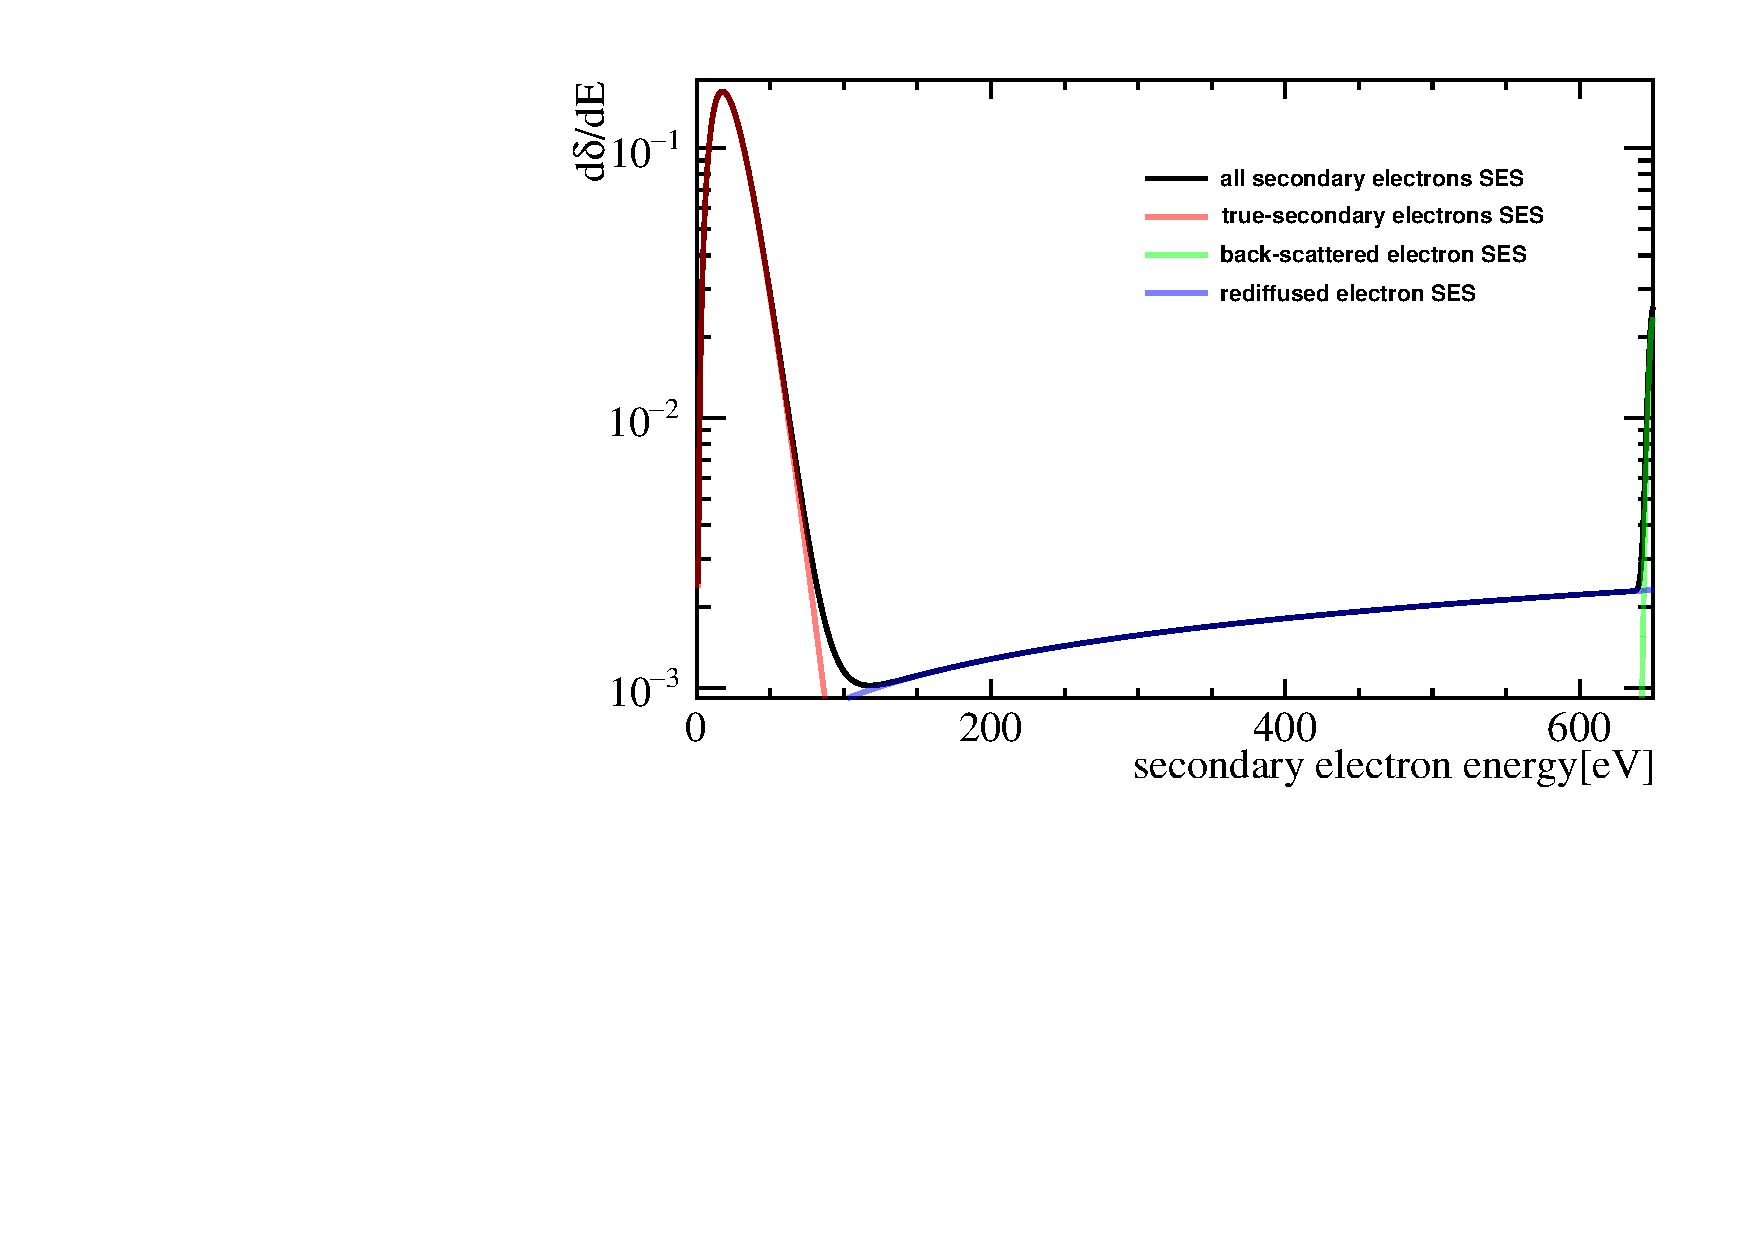
\includegraphics[width=0.6\textwidth]{pic/SES.pdf}
    \caption{When primary energy is \SI{650}{eV},
        the red line represents $d\delta_{\mathrm{bs}}/dE$,
        the blue line represents $d\delta_{\mathrm{rd}}/dE$,
        the green line represents $d\delta_{\mathrm{ts}}/dE$,
        and the black one is $d\delta/dE$.}
    \label{fig:SES}
\end{figure}


\subsection{Voltage-division Experiment}\label{sec:gain}
From Sec.~\ref{subsec:fuman} and as shown in Fig.~\ref{fig:SES},
secondary electrons have lower energies and usually less than \SI{100}{eV} when incident energy is \SI{650}{eV}.
When the primary energy is below \SI{100}{eV}, the SEY is much smaller than which at \SI{650}{eV}~\cite{2012An}.
Thus, the gain of single secondary electron is not the same as the photoelectrons directly entering the channels.
A voltage-division experiment is designed to measure the relationship
between the gains of MCP and the energies of electrons entering the MCP channels.

\subsubsection{Experimental setup}
The energy of the photoelectron arriving at the MCP is almost determined by the voltage difference
between the photocathode and the MCP, based on which we can control the energy of the electrons by adjusting the voltage.
As shown in the Fig.~\ref{fig:setup}, a positive and a negative high voltage supplies are used.
A high sampling rate oscilloscope is used to capture all the waveforms.

As shown in Fig.~\ref{fig:circuit}, an adjustable high voltage between the photocathode and $\mathrm{M}1$ the upper surface of the first MCP
is provided by the negative high voltage power supply.
The positive high voltage power supply delivers 4 consistent voltages to the two MCPs
after being divided by resistors as shown in Fig.~\ref{fig:setup} following the voltage divider designed in~\cite{Luo:2023jdf}.
There is a stable voltage difference between the two MCPs difined as the gap voltage~\cite{2017MCP}.
With this experimental setup,
simultaneously adjusting the electron incident energy
and keeping the voltage division of the MCPs stability are achieved.
This can also be accomplished by using more power supplies~\cite{2017MCP}
which is harder to operate but easier to change the voltage differences of MCPs.
\begin{figure}[ht]
    \centering
    \begin{subfigure}{\textwidth}
        \centering
        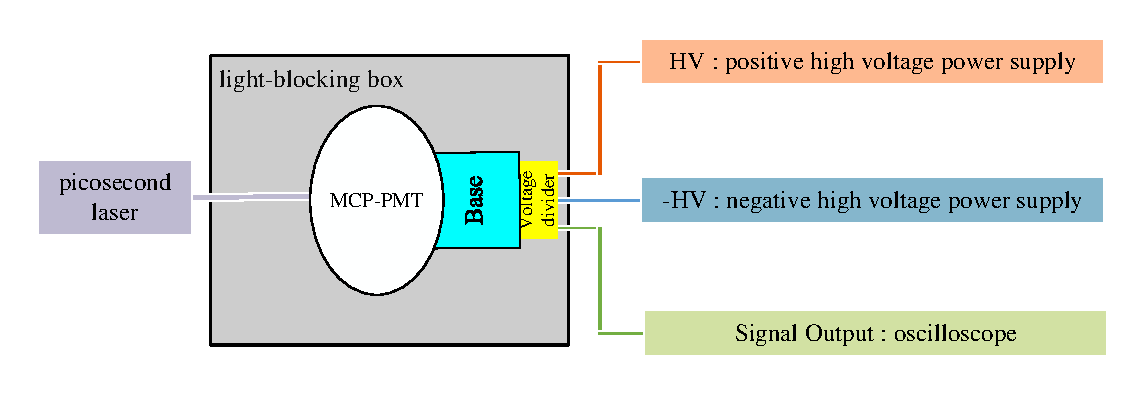
\includegraphics[width=0.7\linewidth]{pic/setup.pdf}
        \caption{}
        \label{fig:setup}
    \end{subfigure}
    \vspace{0.5cm}
    \begin{subfigure}{\textwidth}
        \centering
        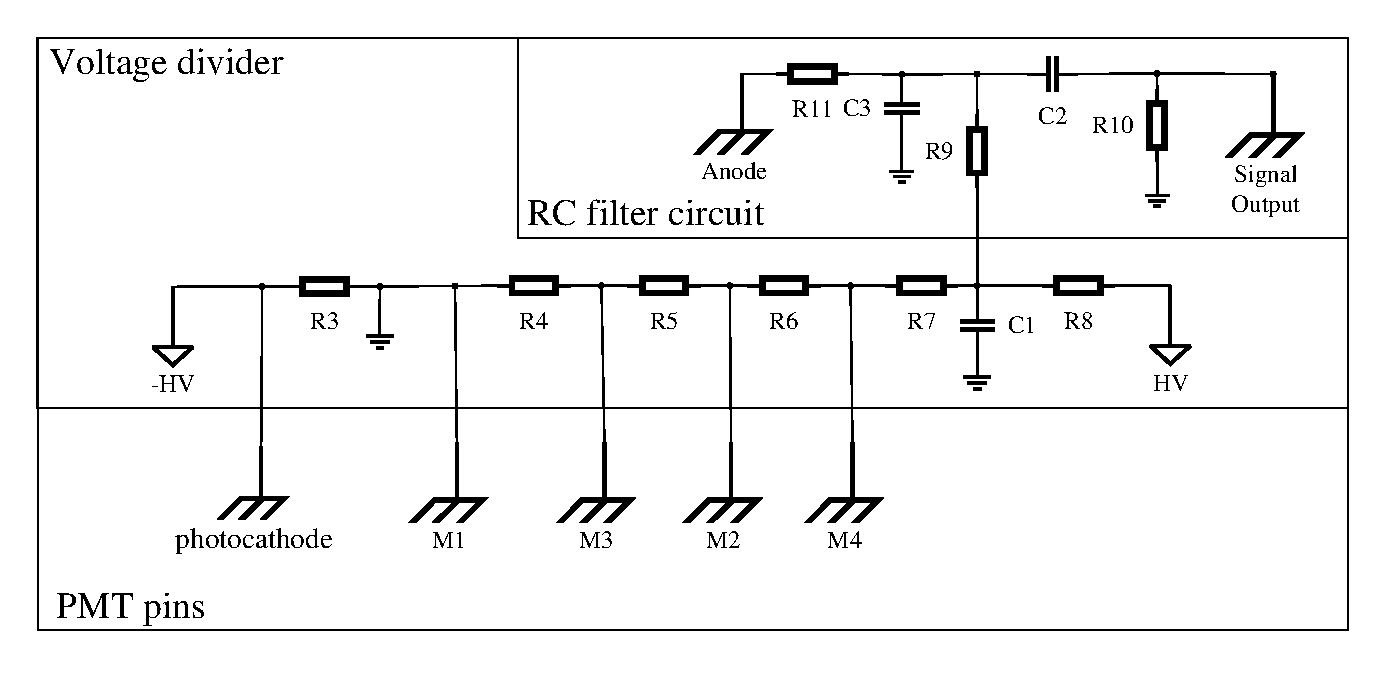
\includegraphics[width=0.7\linewidth]{pic/circuit.pdf}
        \caption{}
        \label{fig:circuit}
    \end{subfigure}
    \caption{Experimental setup and the circuit of voltage divider.
        The plot~\subref{fig:setup} is schematic diagram of the experimental setup:
        simultaneously supply positive and negative high voltages to the MCP-PMT,
        and capture the output waveforms using an oscilloscope.
        The plot~\subref{fig:circuit} is the experimental circuit diagram:
        supply the photocathode with the negative high voltage,
        supply the two MCPs with the positive high voltage,
        and use an RC filtering and shaping circuit
        to convert the amplified electrical signal into waveforms output.
        $\mathrm{M}1$, $\mathrm{M}3$ are the upper surfaces of MCPs
        and $\mathrm{M}2$, $\mathrm{M}4$ are the lower surfaces.
        The gap voltage is between $\mathrm{M}2$ and $\mathrm{M}3$.}
    \label{fig:mainfig}
\end{figure}

\subsubsection{Relationship of gain and incident energy}
A new waveform analysis method named fast stochastic matching pursuit~(FSMP)~\cite{Xu_2022}
utilizing Markov Chain Monte Carlo is employed. With the best accurate time and intensity resolution,
FSMP provides more precise measurements of SER charge spectrum.

To exclude the influence of the surface mode, we conducted the same test on MCP-PMTs with and without ALD coating.
\begin{figure}[ht]
    \centering
    \begin{subfigure}[b]{0.48\textwidth}
        \centering
        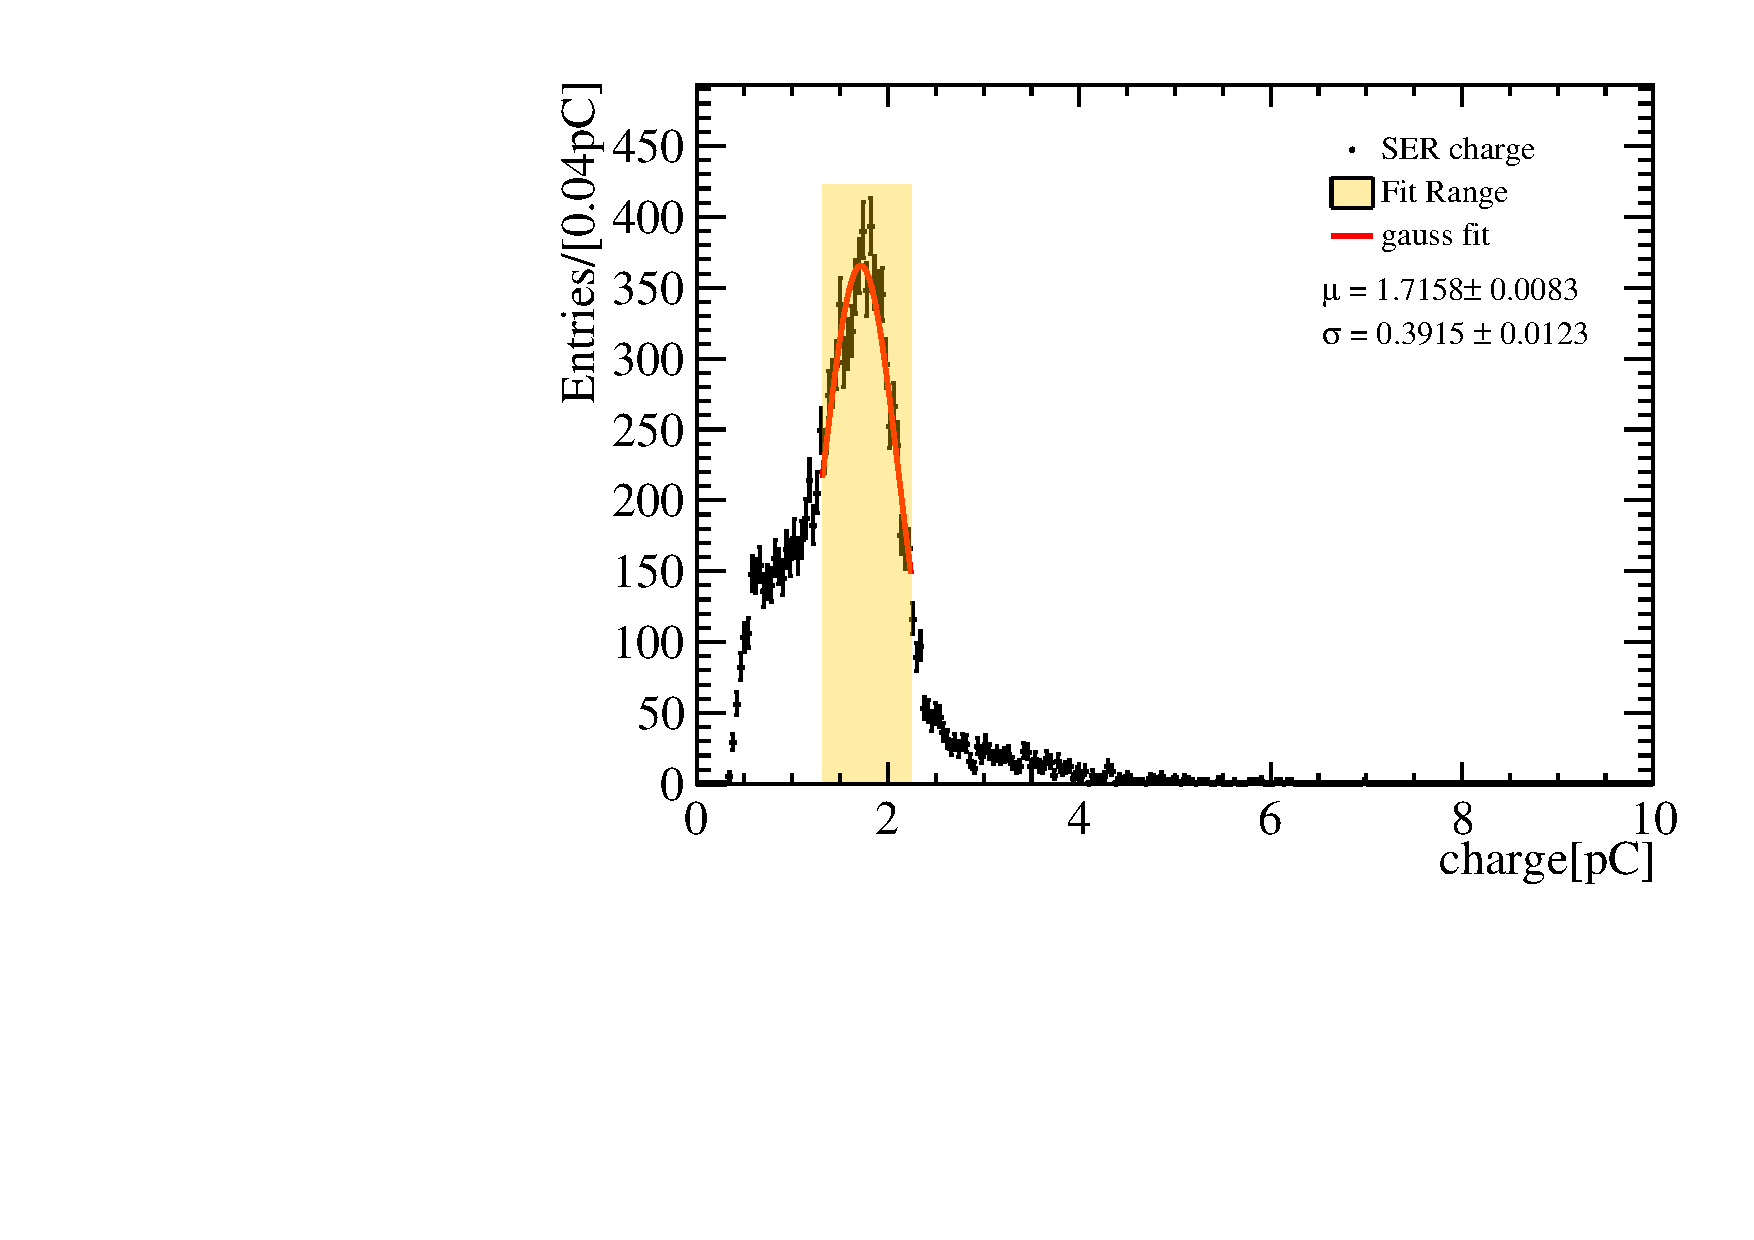
\includegraphics[width=\textwidth]{pic/SER_noALD.pdf}
        \caption{}
        \label{fig:gain_noald}
    \end{subfigure}
    \hfill
    \begin{subfigure}[b]{0.48\textwidth}
        \centering
        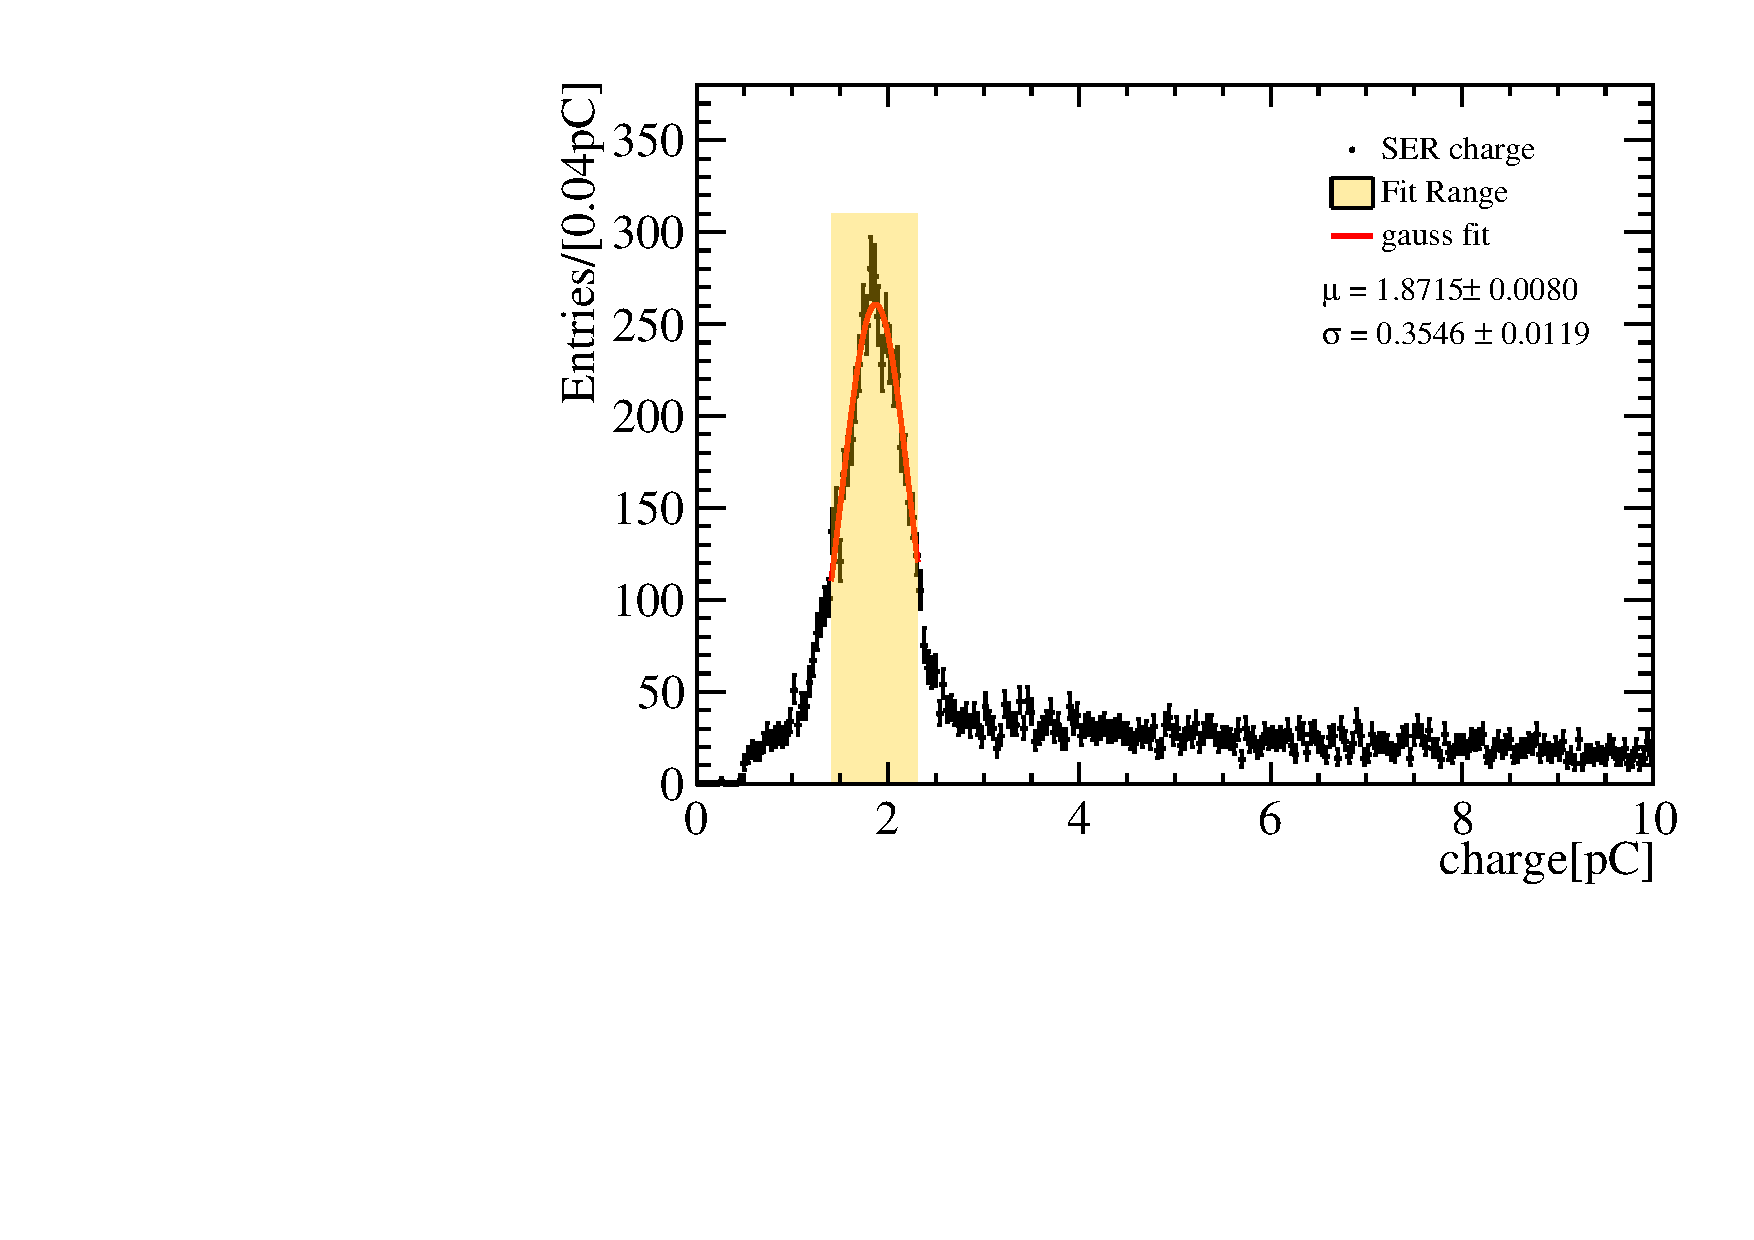
\includegraphics[width=\textwidth]{pic/SER_ALD.pdf}
        \caption{}
        \label{fig:gain_ald}
    \end{subfigure}
    \caption{The plot~\subref{fig:gain_noald} displays the fit of the charge spectrum of the MCP-PMT without ALD coating,
        while the plot~\subref{fig:gain_ald} shows the fit with ALD coating.
        We observed that the plot~\subref{fig:gain_noald} does not exhibit large charges.}
    \label{fig:gain_fit}
\end{figure}
The $\mu$ and $\sigma$ are calculated for every initial energy
by fitting the main peak of SER charge spectra with Gaussian distribution as shown in Fig.~\ref{fig:gain_fit},
$g_{\mathrm{\mu,\sigma}}(E)$ is the function to describe the relationship between gains and electron energies as shown in Fig.~\ref{fig:gaintest}.

\begin{figure}[ht]
    \centering
    \begin{subfigure}[b]{0.48\textwidth}
        \centering
        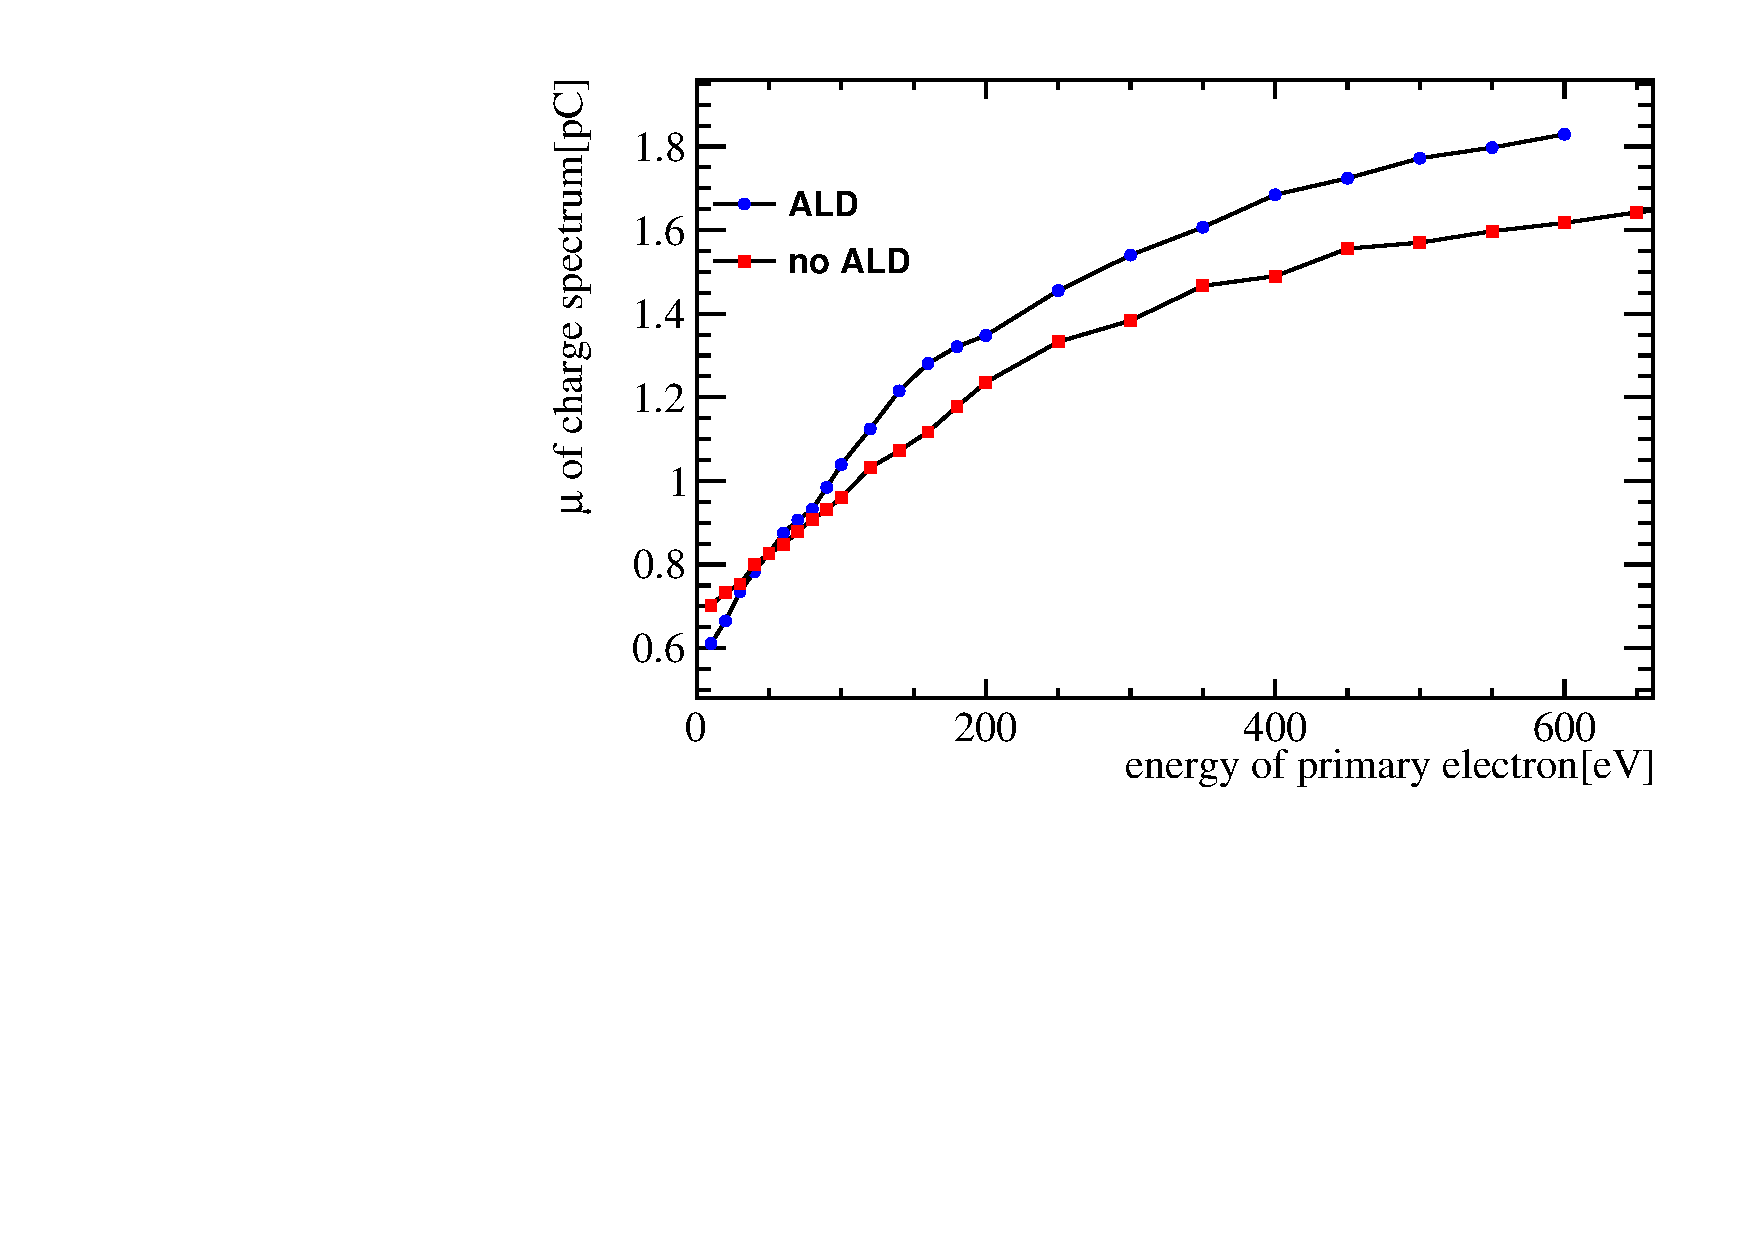
\includegraphics[width=\textwidth]{pic/gain.h5_mu.pdf}
        \caption{}
        \label{fig:gain}
    \end{subfigure}
    \hfill
    \begin{subfigure}[b]{0.48\textwidth}
        \centering
        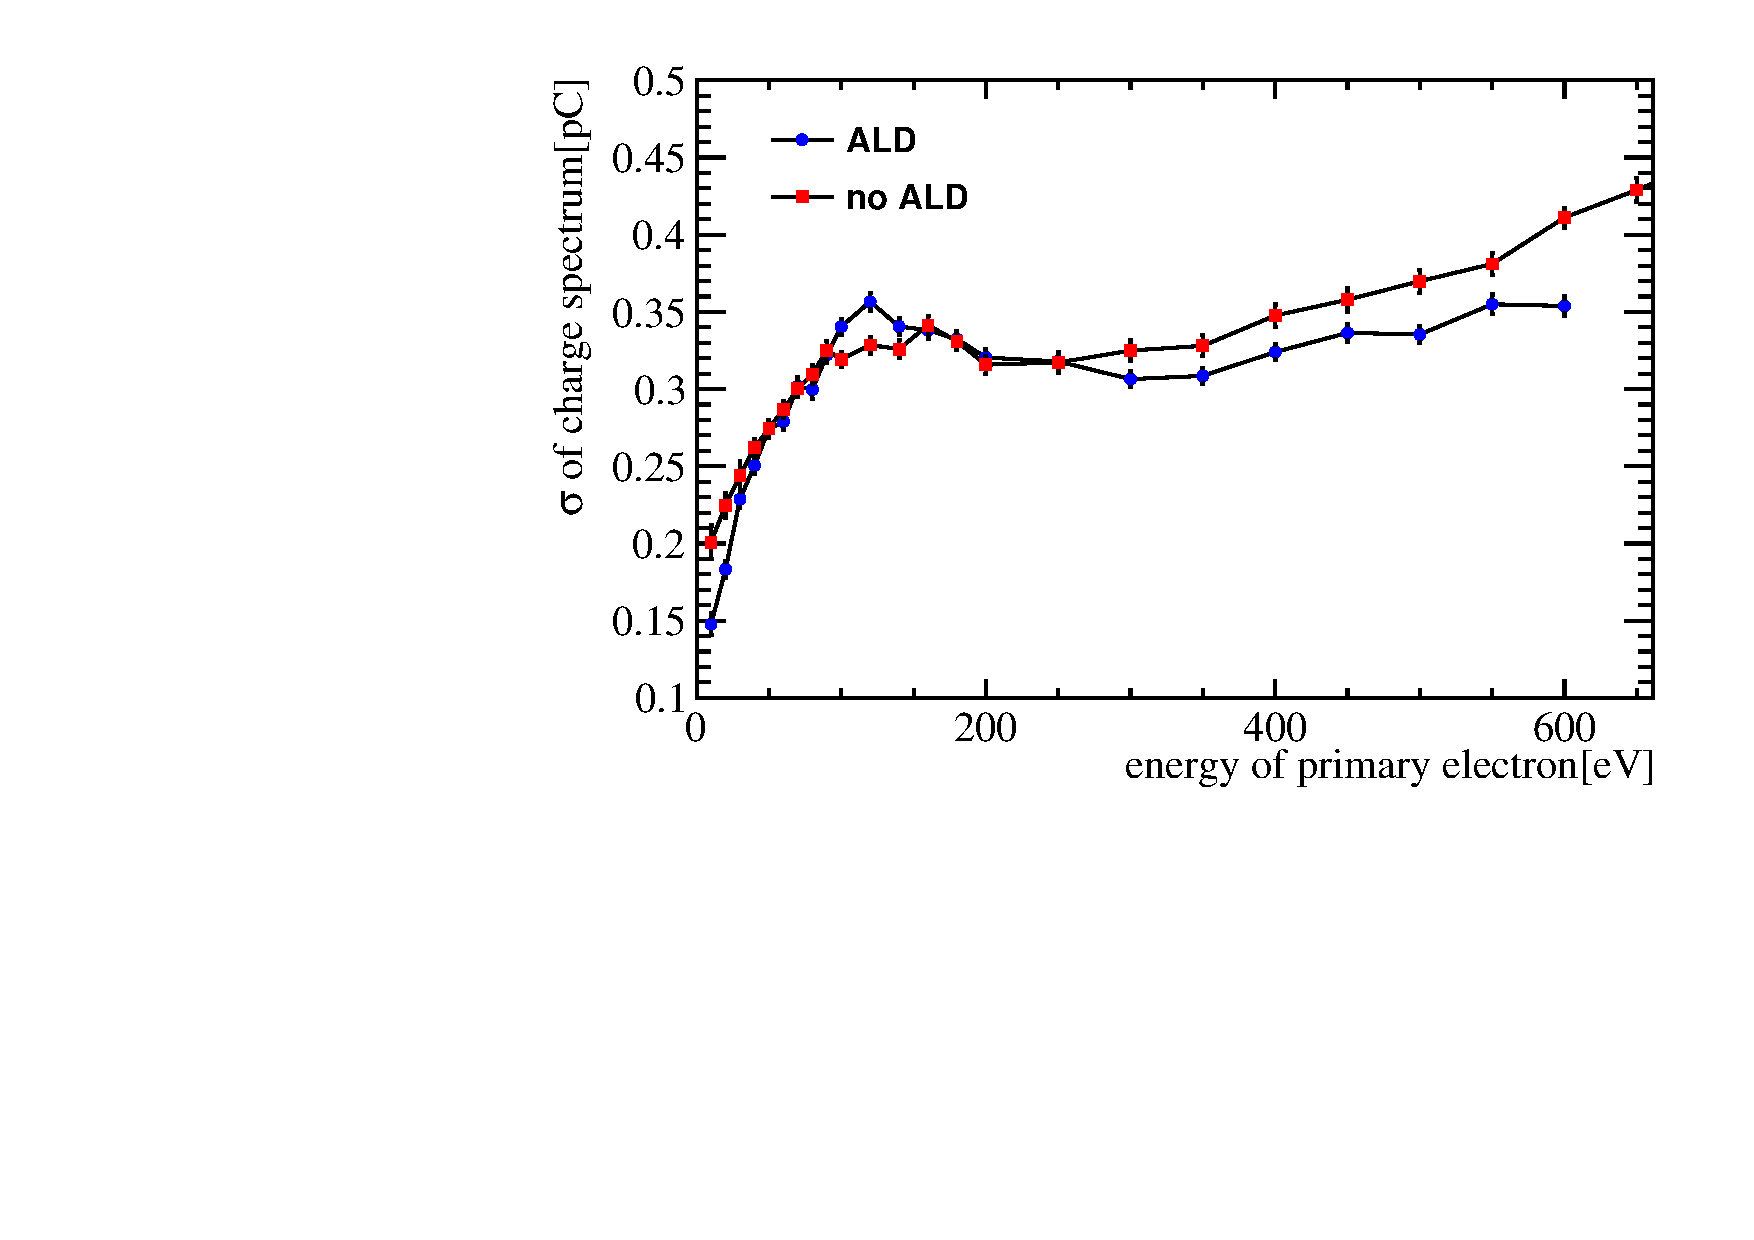
\includegraphics[width=\textwidth]{pic/gain.h5_sigma.pdf}
        \caption{}
        \label{fig:sigma}
    \end{subfigure}
    \caption{The plot~\subref{fig:gain} shows that the mean increases as initial electron energy increases,
        and the plot~\subref{fig:sigma} shows the variance changes with energy.
        MCP-PMT with ALD coating~(the red line) shows a similar variation trend to the one without ALD coating~(the blue line).}
    \label{fig:gaintest}
\end{figure}

When the electron energy is less than \SI{400}{eV} , the gain rapidly increases with the electron energy.
As the electron energy reaches \SI{400}{eV}, the gain gradually stabilizes.
Similar results are reported in~\cite{2017MCP}.
The gains for the low-energy secondary electrons
from the surface mode are lower than that from channel mode.

The charge responses of electrons with different energies are superimposed
according to the SES to obtain the charge response of the surface mode.

\subsection{Monte Carlo calculation}\label{sec:convolution}
Note the probability of electrons directly entering the channel and hitting on the MCP upper surface as $p$ and $1-p$.
Considering that the number of secondary electrons~$n_{\mathrm{se}}$ may exceed 1,
The SER charge can be described as Eq.~\eqref{eq:convolution},
\begin{equation}
    \label{eq:convolution}
    \begin{aligned}
        Q_{\mathrm{MCP-PMT}} & = p\times Q_{\mathrm{channel}}+(1-p)\times Q_{\mathrm{surface}}                                                            \\
                             & = p\times Q_{\mathrm{channel}}+(1-p)\times \frac{\int_0^{E_0}G(E)f_{\mathrm{SES}}(E)dE}{\int_0^{E_0}f_{\mathrm{SES}}(E)dE} \\
    \end{aligned}
\end{equation}
where $Q_{\mathrm{MCP-PMT}}$ is the SER charge distribution of MCP-PMT,
$Q_{\mathrm{channel}}$ and $Q_{\mathrm{surface}}$ are the charge distributions of the charge mode and the surface mode,
and $G(E)$ whose parameters are taken from $g_{\mathrm{\mu,\sigma}}$ is the charge distribution when incident energy is $E$.
The SER charge distribution is simulated using Monte Carlo method~\cite{1951Various} as shown in Fig.~\ref{fig:process}.
The probabilities of the three processes are approximated by the relative amounts of the yields.
For true-secondary electrons, their number $n$ is given by Poisson sampling and the sum of the sampled $n$ charges
serves as the output charge.
\begin{figure}[ht]
    \centering
    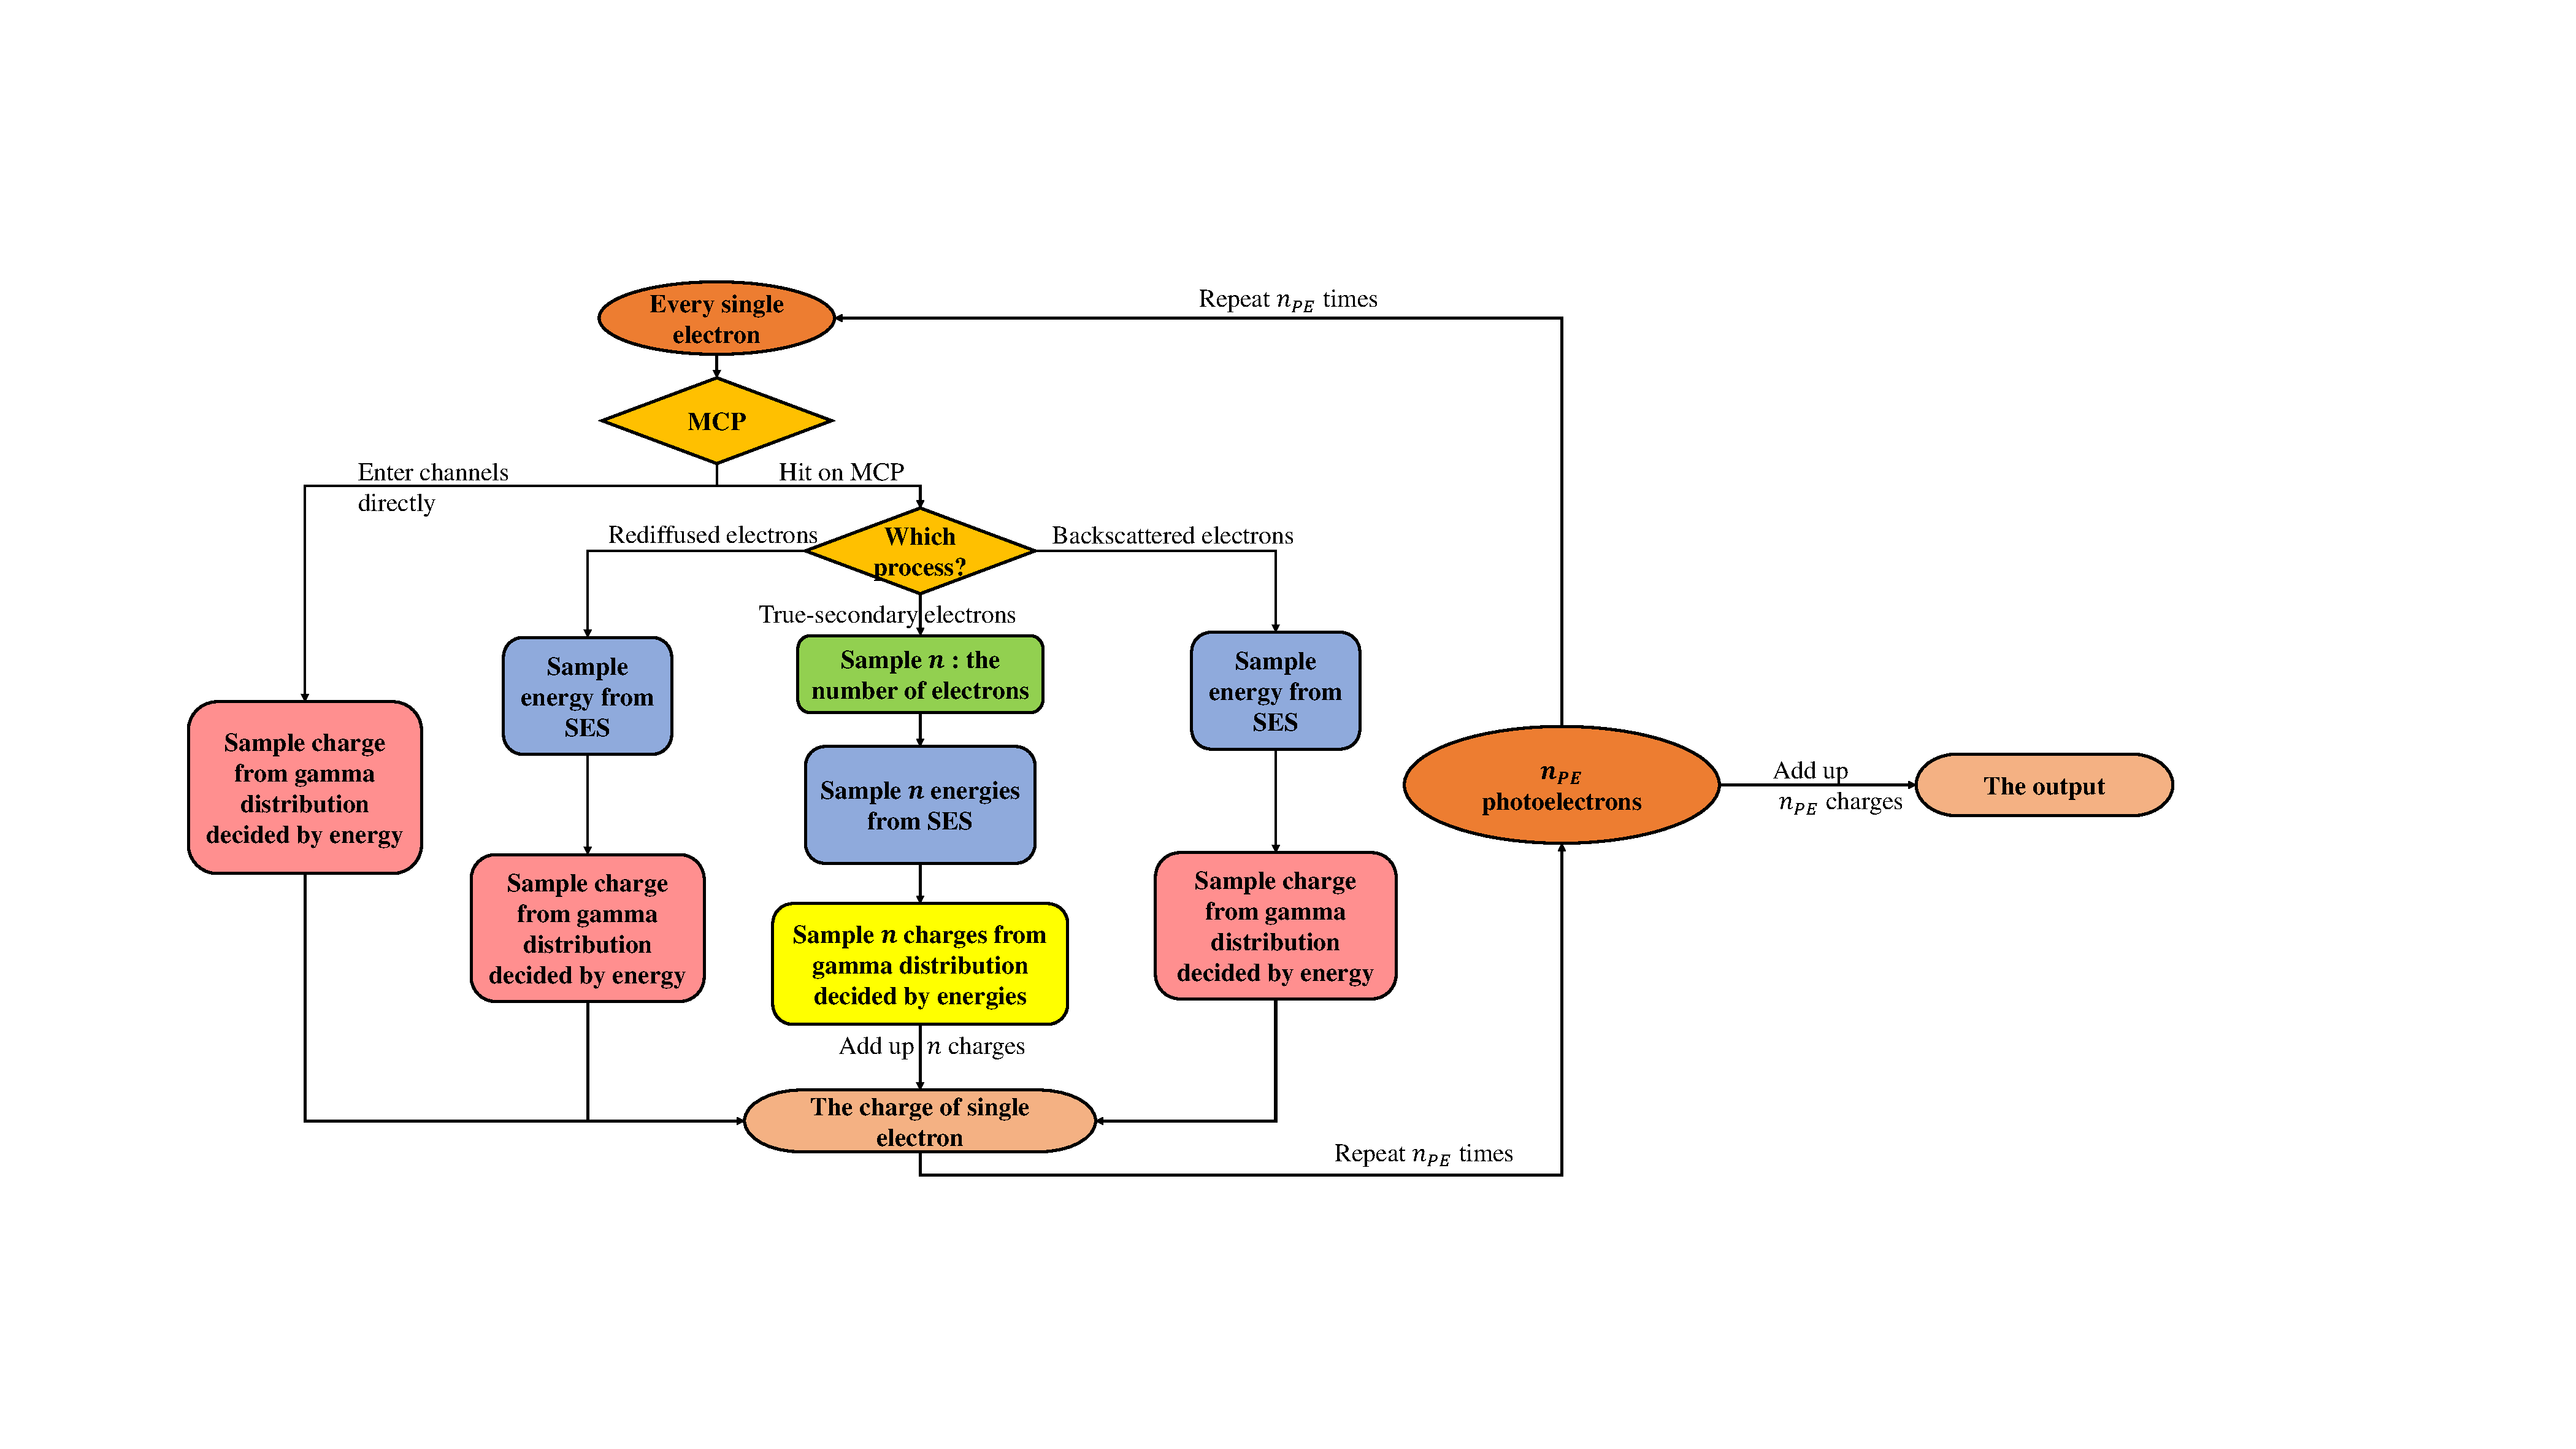
\includegraphics[width=0.95\linewidth]{pic/process.pdf}
    \caption{The procedure of Monte Carlo method for computing the SER charge spectrum.}
    \label{fig:process}
\end{figure}
Through the procedure, the charge response generated by a single electron incoming and by $n_{\mathrm{PE}}$ are calculated.
\begin{figure}[ht]
    \centering
    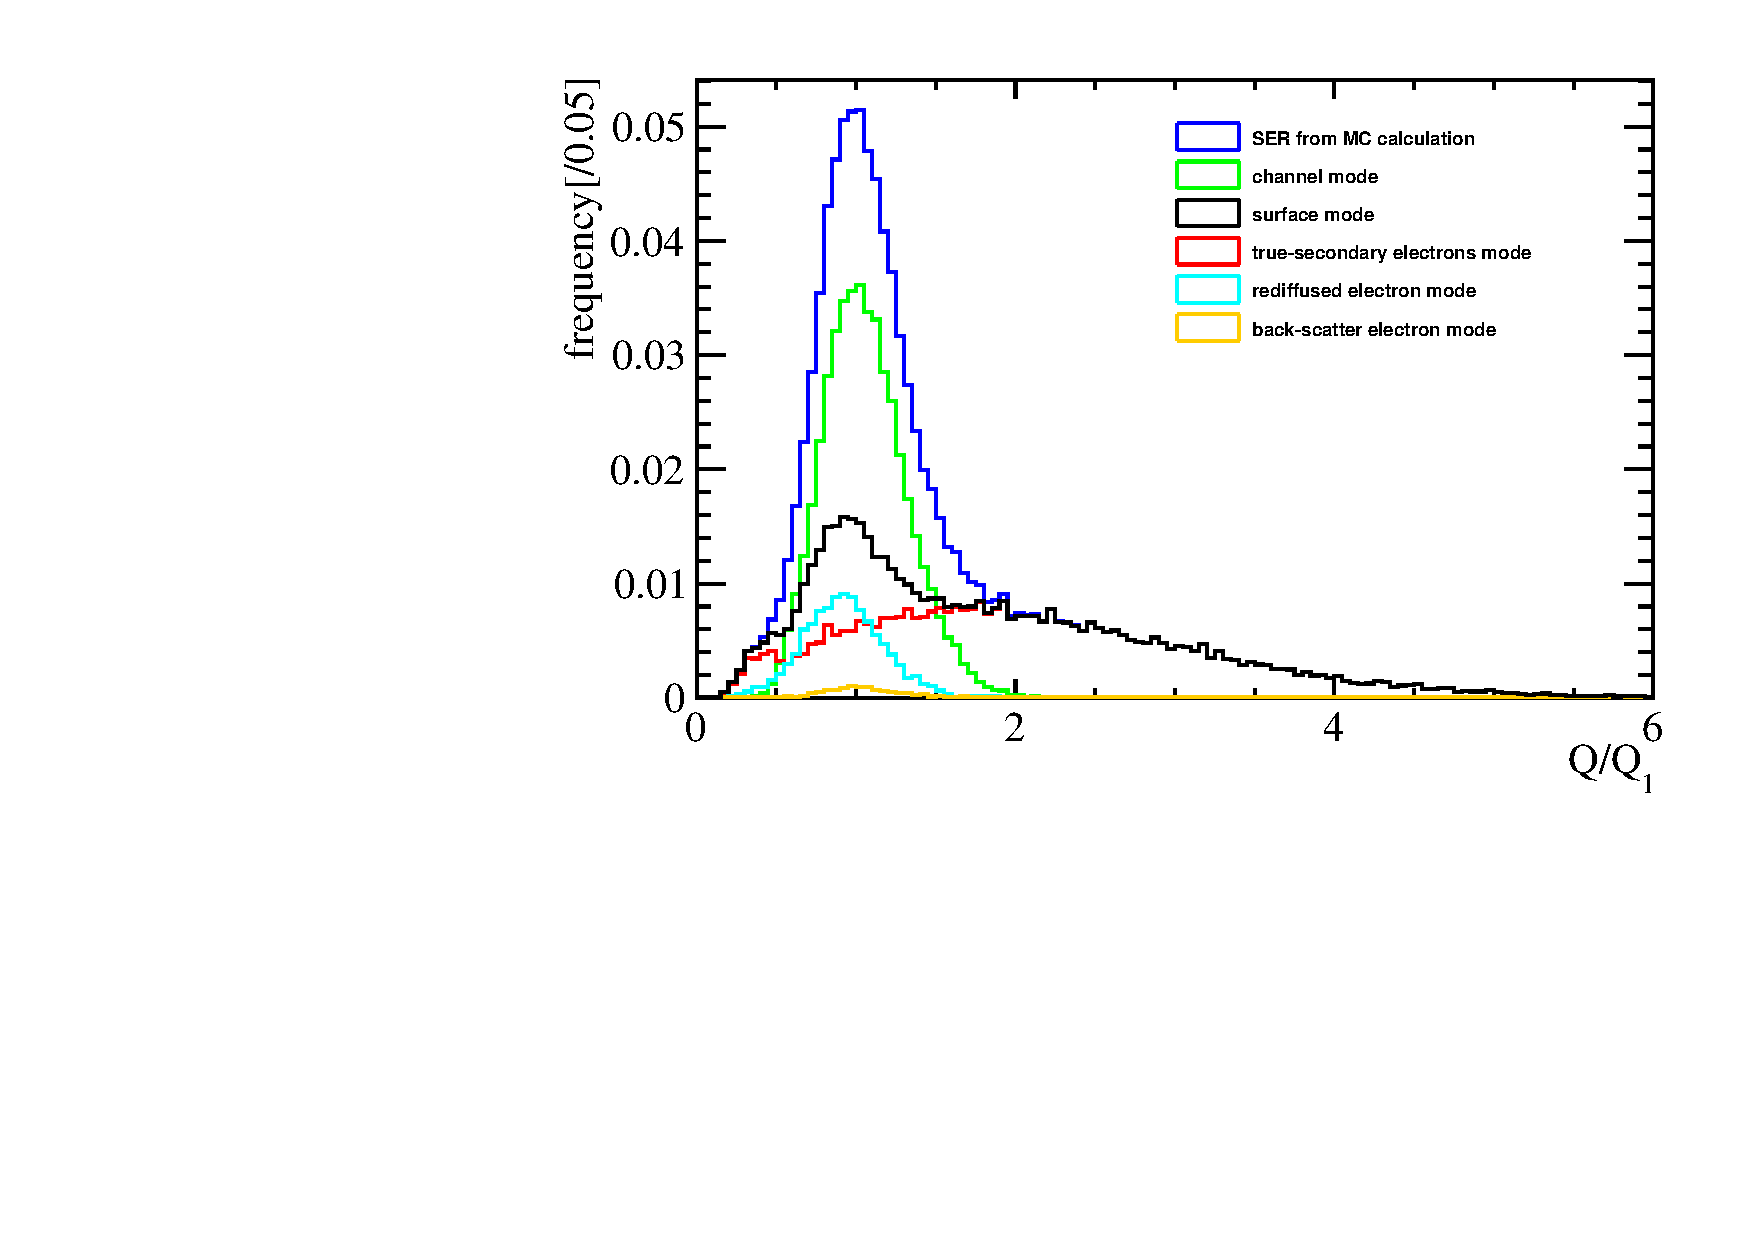
\includegraphics[width=0.6\linewidth]{pic/allmode.pdf}
    \caption{The charge distribution formed in the channel mode is concentrated around the main peak,
        while the tail portion is mainly generated by the true-secondary electrons in the surface mode.}
    \label{fig:allmode}
\end{figure}
The charge distribution of the surface mode can be divided into three components according to the Furman model,
the back-scattered electron mode defined as $Q_{\mathrm{bs}}$,
the rediffused electron mode defined as $Q_{\mathrm{rd}}$,
and the true-secondary electrons mode defined as $Q_{\mathrm{ts}}$.
\begin{equation}
    \label{eq:surface_3}
    Q_{\mathrm{surface}} = Q_{\mathrm{ts}}+Q_{\mathrm{rd}}+Q_{\mathrm{bs}}
\end{equation}

The back-scattered electron mode is predominantly distributed at the main peak,
while the rediffused electron mode exhibits a distribution in close proximity to the main peak.
These two components within the surface mode contribute to a single secondary emission electron.
There exists little difference in energy between in the channel mode and in the back-scattered electron mode
resulting in that the amplified charge is basically the same.
Due to the energy of the rediffused electron slightly lower than that in the channel mode,
the amplified charge after MCP multiplication is slightly smaller.
Therefore, the contribution of these two modes to the large charges in SER charge spectrum can be considered negligible.

In the true-secondary electrons mode, the charge can be described as Eq.~\eqref{eq:ts_all}:
\begin{equation}
    \label{eq:ts_all}
    \begin{aligned}
         & Q_{\mathrm{ts}} = \sum_{n=0}^{\infty} \sum_{i=0}^{n} Q_{\mathrm{i}}      \\
         & Q_{\mathrm{i}} \sim \varGamma  (\alpha_{\mathrm{i}}, \beta_{\mathrm{i}}) \\
         & n \sim \mathrm{\pi}(\delta_{\mathrm{ts}})
    \end{aligned}
\end{equation}
\begin{figure}[ht]
    \centering
    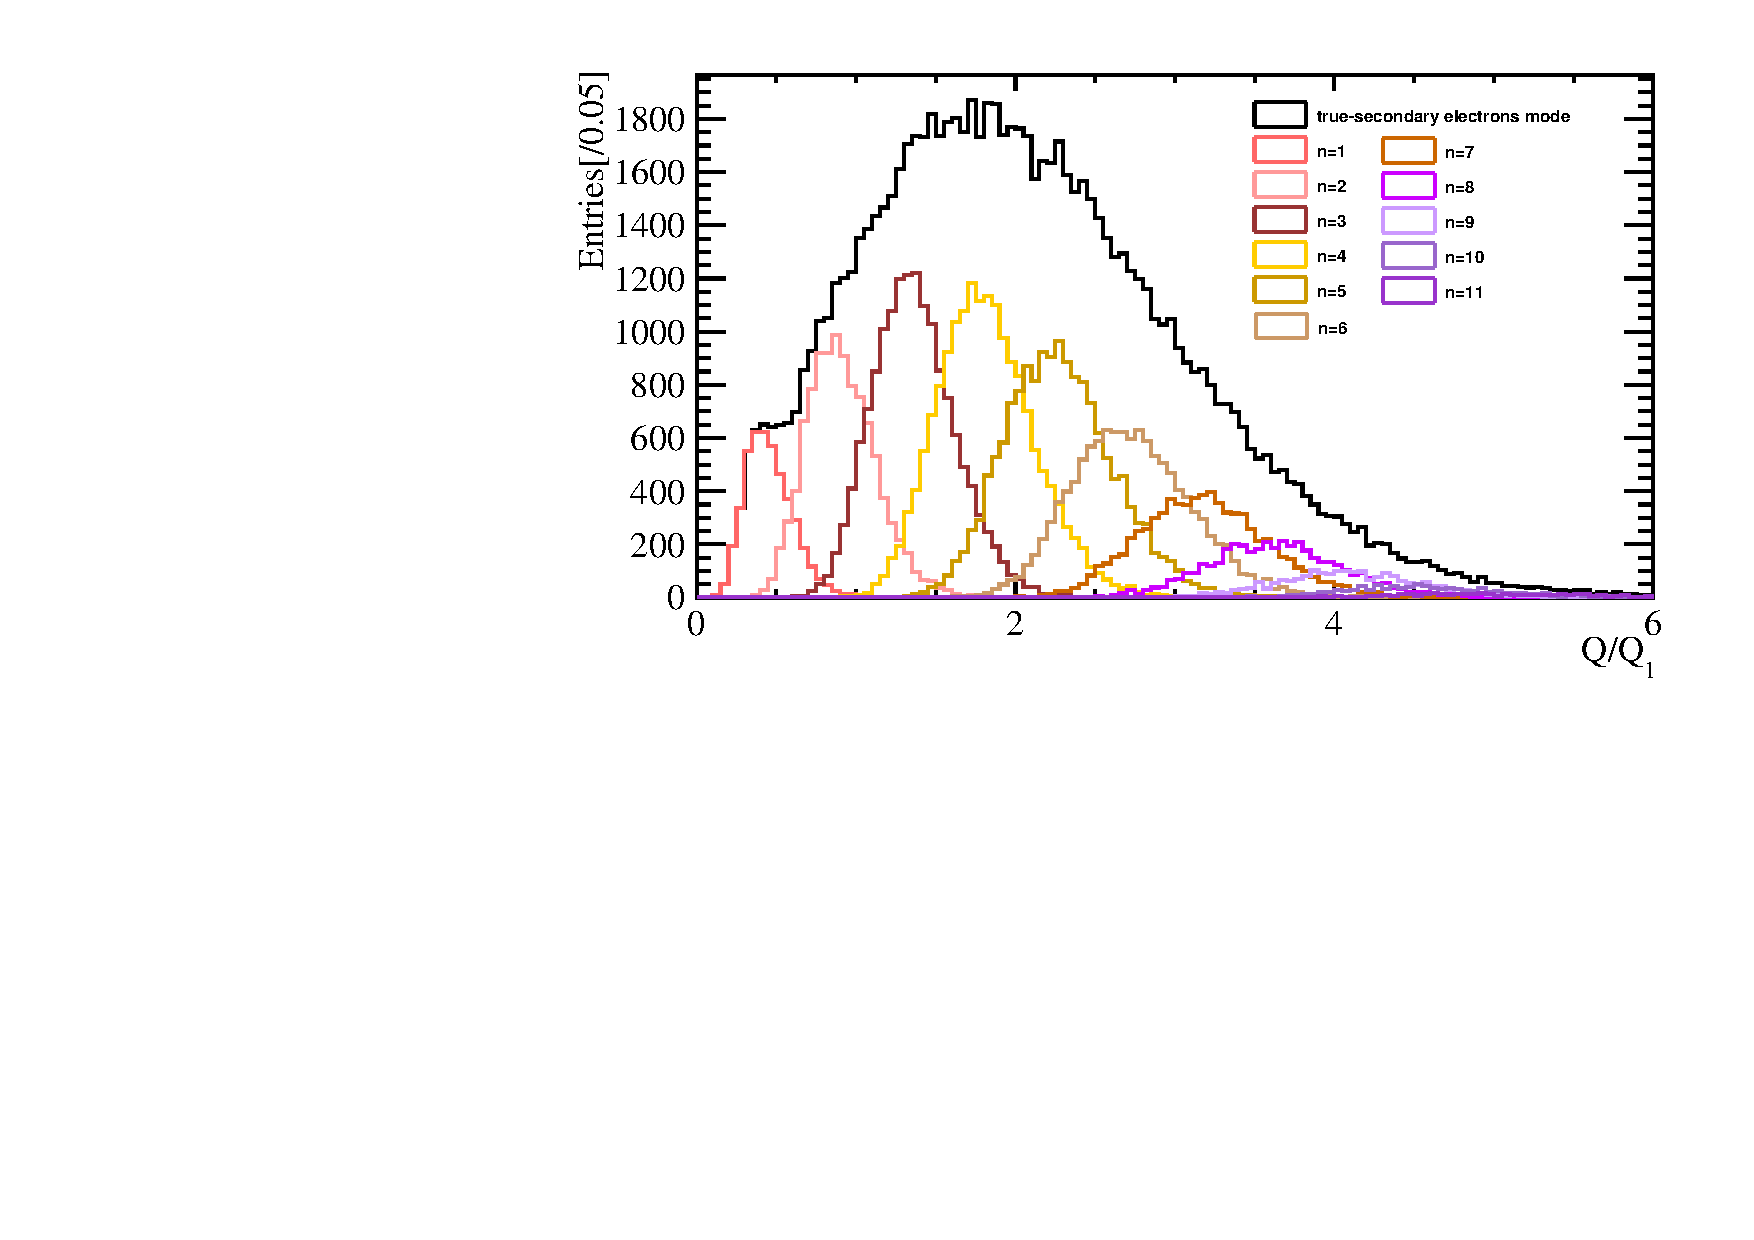
\includegraphics[width=0.6\linewidth]{pic/true_all.pdf}
    \caption{The charge distribution of true-secondary electrons mode in MC calculation when $\delta_{\mathrm{ts}}=4.5$ and $p=0.5$.
        The black histogram is the total distribution consisting of the histograms for different $n$.}\label{fig:true_n}
\end{figure}

The charge spectrum of different $n$ is shown in Fig.~\ref{fig:true_n}.
For each photoelectron in true-secondary electrons mode,
the output is the sum of the $n$ charges and the bigger $n$ is, the larger the charge is.
Due to the lower energy of the generated electrons,
the charge after each electron multiplication is smaller.
It is challenging to distinguish the multiplied charges formed at the anode,
as multiple secondary electrons are generated and enter the MCP channels simultaneously.
Their combined form results in a larger charge formation,
contributing to the "long-tail" of the SER charge spectrum.


\subsection{Tuning model with experiment data}\label{subsec:chitest}
The field $\delta_{\mathrm{ts}}$ of the true-secondary electrons and the probability $p$ in Eq.~\eqref{eq:convolution}
which have a significant impact on the SER charge distribution as shown in Fig.~\ref{fig:tsp} are selected
to generate different histograms by MC.
\begin{figure}[ht]
    \centering
    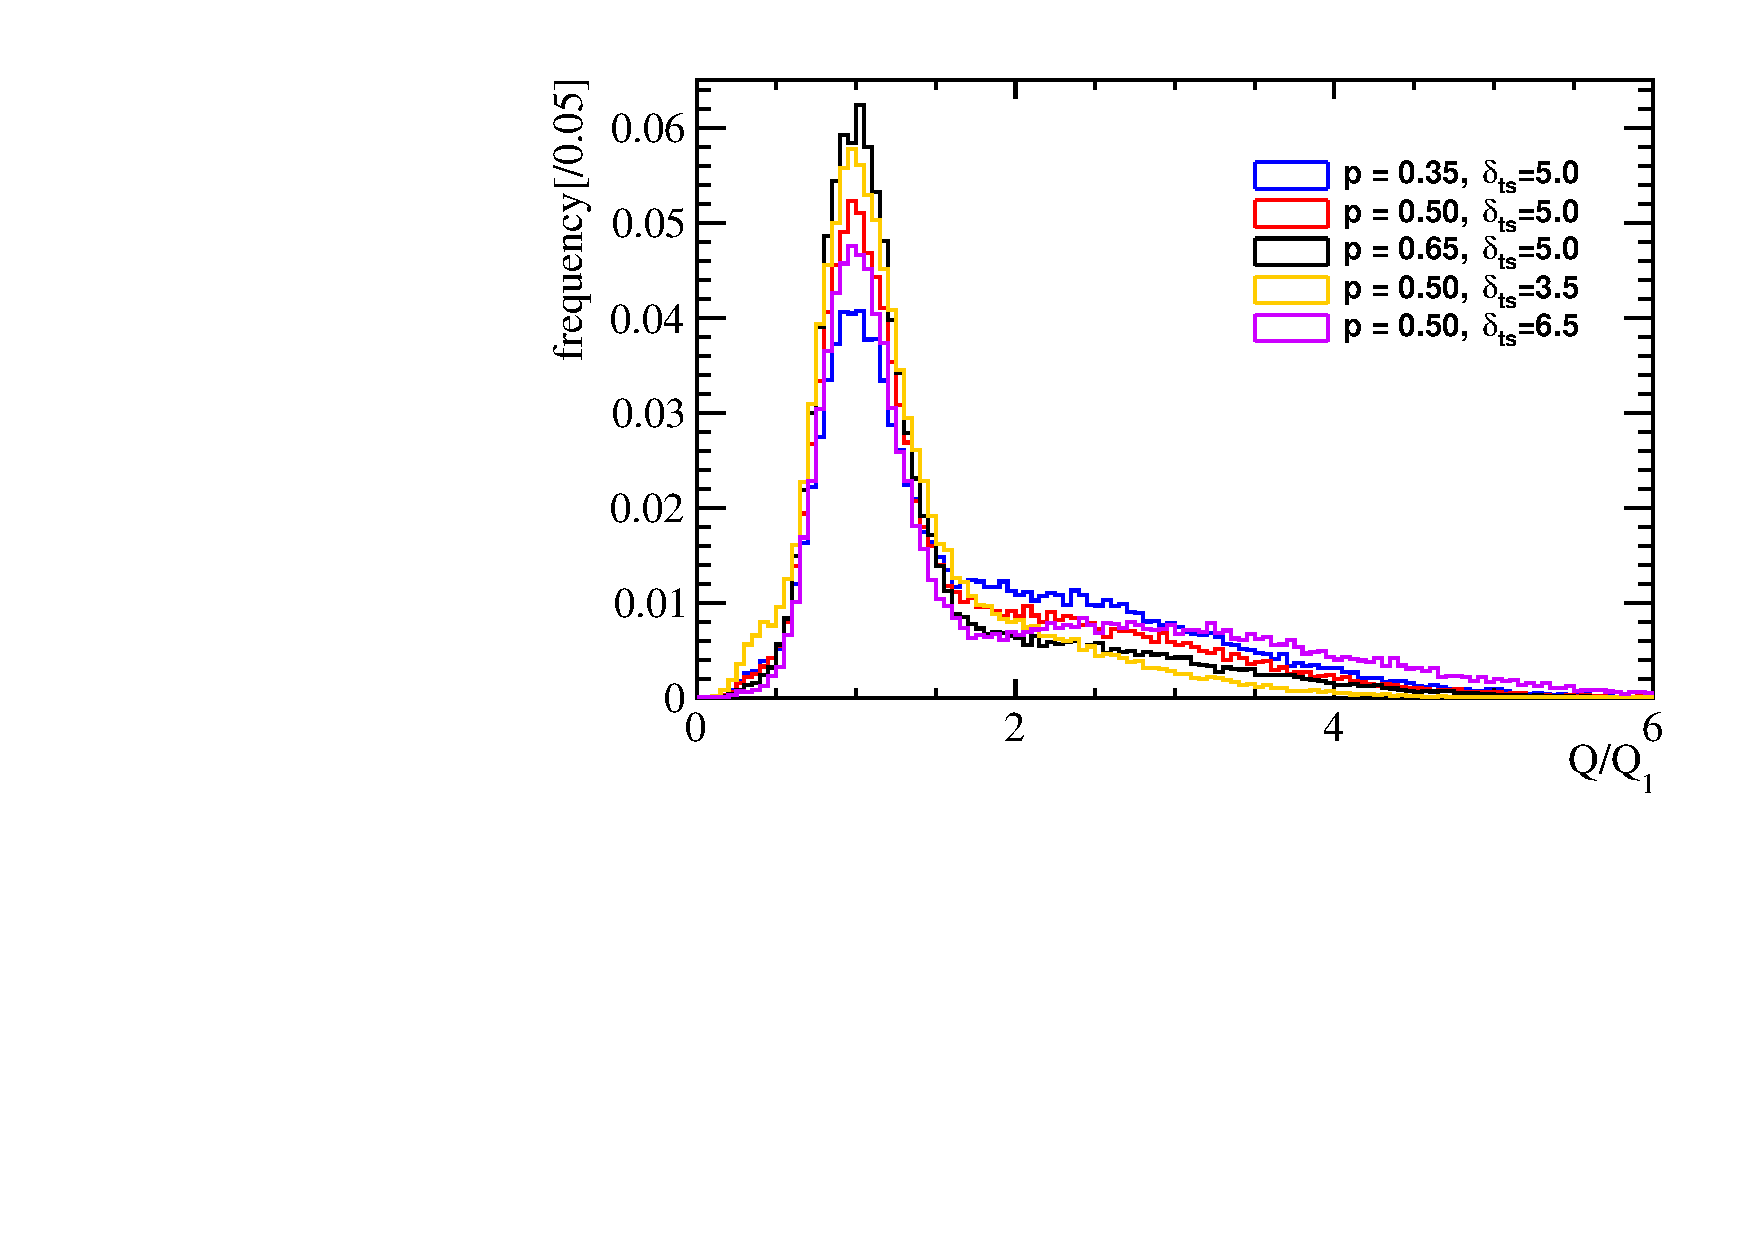
\includegraphics[width=0.6\linewidth]{pic/pts.pdf}
    \caption{The shape of SER charge spectrum from MC is influenced by $\delta_{\mathrm{ts}}$ and $p$.
        As $\delta_{\mathrm{ts}}$ increases gradually, the height of the main peak region the tail gradually becomes longer and bigger.
        As $p$ gradually increases, the height of the main peak region increases, and the tail gradually becomes narrower
    }
    \label{fig:tsp}
\end{figure}

A chi-square test is then performed between each
MC histogram and the histogram of single photoelectron charge obtained from the MCP-PMT test.
The histograms of MC and test have the same binning with the number of bins being $r$.
The entries in i-th bin are $n_{\mathrm{i}}$ and $m_{\mathrm{i}}$; total entries are
$N = \sum_{{\mathrm{i}}=1}^{r}n_{\mathrm{i}}$ and $M = \sum_{{\mathrm{i}}=1}^{r}m_{\mathrm{i}}$.
The chi-square test indicates the similarity between two histograms, with chi-square defined in Eq.~\eqref{eq:chi}~\cite{2006Comparison}.
The chi-squares between the histograms of MC and experiment data are scanned in the $p-\delta_{\mathrm{ts}}$ grid as shown in Fig.~\ref{fig:cour}.
The distribution of the chi-square
with respect to $p$ and $\delta_{\mathrm{ts}}$ is continuous,
and a linear regression can be used to fit the relationship
between chi-square and $p$ and $\delta_{\mathrm{ts}}$~\cite{oh2013introduction}.
For each MCP-PMT, the parameters corresponding to the minimum chi-square value are selected as the result.
The confidence interval for the parameters can be determined accordingly
with a confidence level of 68.3\%~\cite{cowan1997statistical}.
\begin{equation}
    \label{eq:chi}
    \begin{aligned}
         & \chi^2_{(r-1)}=\sum_{i=1}^r \frac{\left(n_{\mathrm{i}}-N \hat{k}_{\mathrm{i}}\right)^2}{N \hat{k}_{\mathrm{i}}}+\sum_{i=1}^r
        \frac{\left(m_{\mathrm{i}}-M \hat{k}_{\mathrm{i}}\right)^2}{M \hat{k}_{\mathrm{i}}}=\frac{1}{M N} \sum_{i=1}^r
        \frac{\left(M n_{\mathrm{i}}-N m_{\mathrm{i}}\right)^2}{n_{\mathrm{i}}+m_{\mathrm{i}}}                                          \\
         & \hat{k}_{\mathrm{i}}=\frac{n_{\mathrm{i}}+m_{\mathrm{i}}}{N+M}
    \end{aligned}
\end{equation}

\begin{figure}[ht]
    \centering
    \begin{subfigure}{0.47\textwidth}
        \centering
        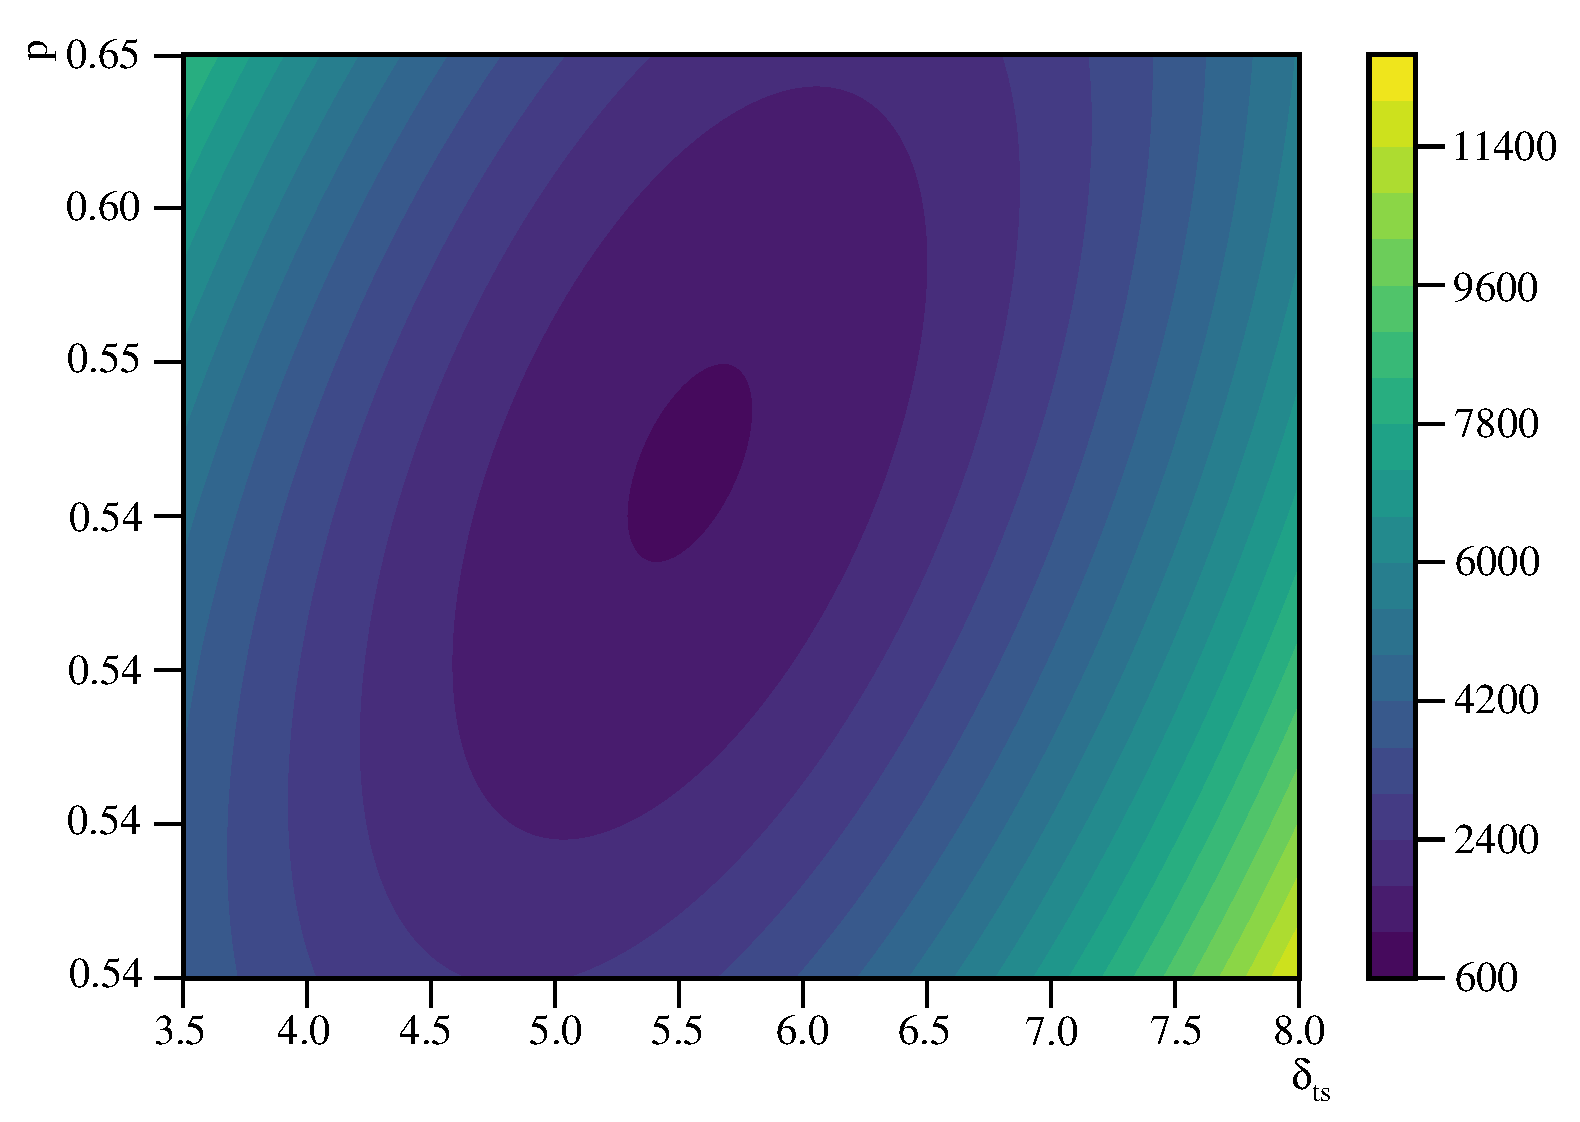
\includegraphics[height=5cm]{pic/cour.pdf}
        \caption{}
        \label{fig:cour}
    \end{subfigure}
    \hfill
    \begin{subfigure}{0.47\textwidth}
        \centering
        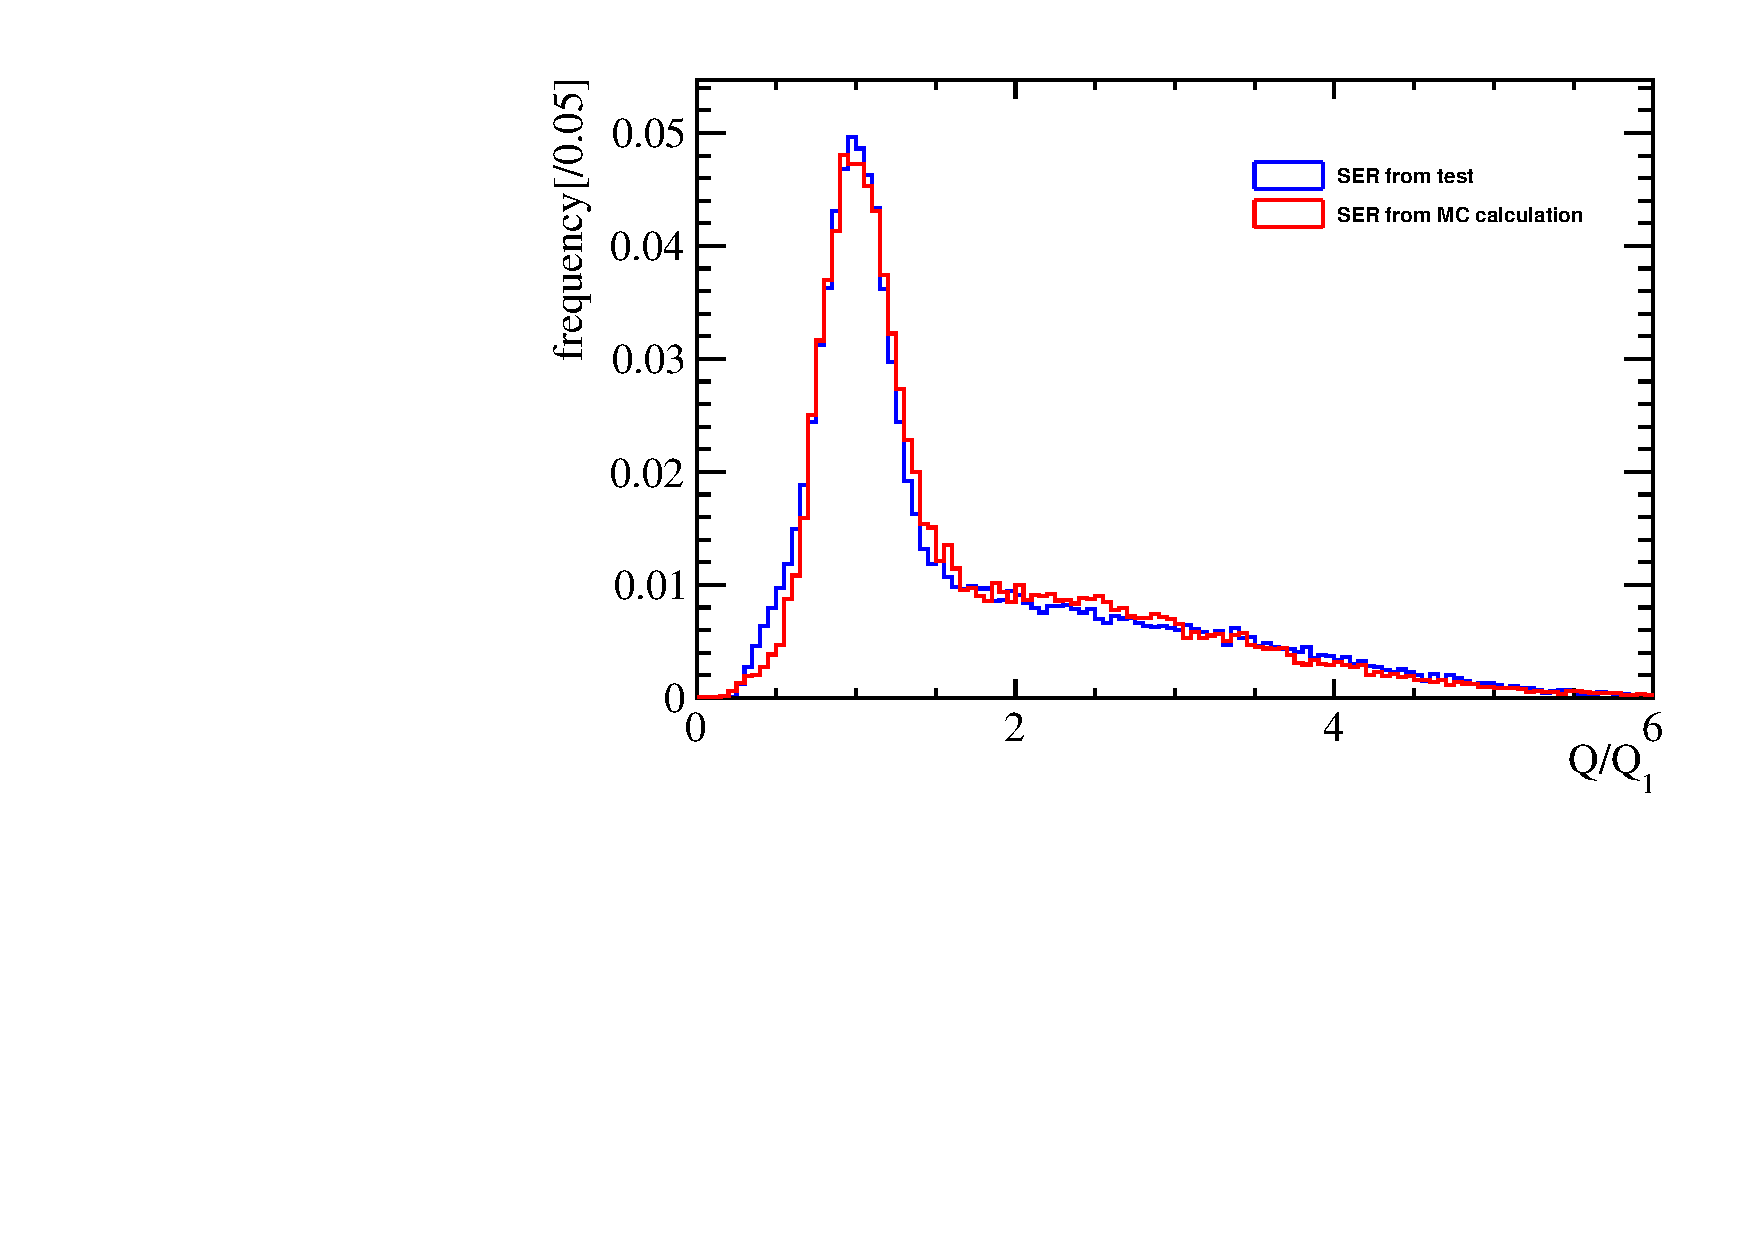
\includegraphics[height=5cm]{pic/hist.pdf}
        \caption{}
        \label{fig:hist}
    \end{subfigure}
    \caption{The plot~\subref{fig:cour} is the contour plot of the chi-square test, with $p$ and $\delta_{\mathrm{ts}}$ as parameters
        and the chi-square values as the height.
        The plot~\subref{fig:hist} is an example of the MC histogram~(the red line) and the histogram from test~(the blue line).
    }
    \label{fig:chi}
\end{figure}

The scatter plot of the $\delta_{\mathrm{ts}}$ and $p$ of 9 MCP-PMTs at the minimum
chi-square is shown in Fig.~\ref{fig:true_p}. The mean of $\delta_{\mathrm{ts}}$
is 5.98 and of $p$ is 0.531, which means that on average,
0.531 electrons directly enter the channel of the MCP.
For each electron incident on the surface of the MCP,
5.98 true-secondary electrons are multiplied.
\begin{figure}[H]
    \centering
    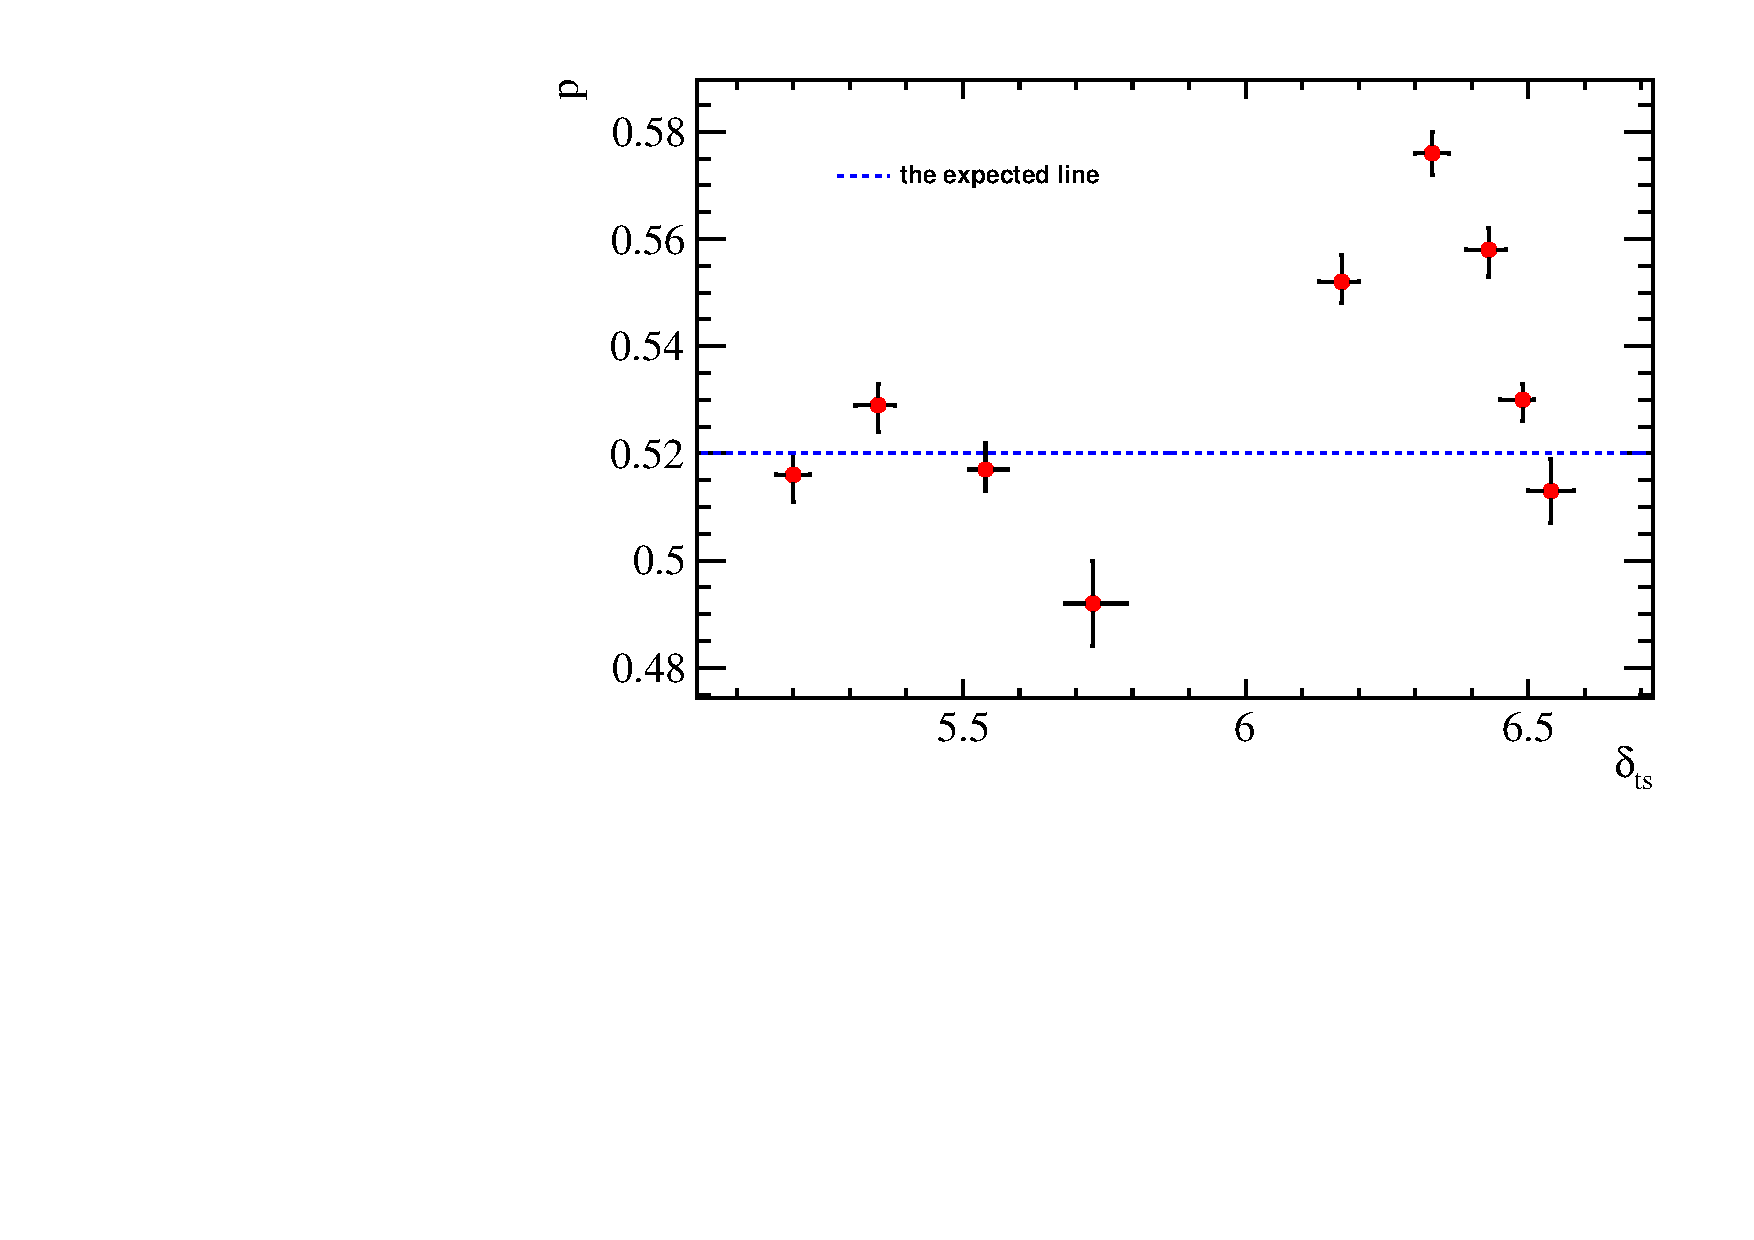
\includegraphics[width=0.6\textwidth]{pic/true_p.pdf}
    \caption{When convolving with 9 MCP-PMTs,
        the distribution of $\delta_{\mathrm{ts}}$ and $p$ at the minimum chi-square
        occurs. The blue dashed line shows the expected $p$.}
    \label{fig:true_p}
\end{figure}

The MCP open area fraction of the MCP-PMT used in JNE is around 65\%
which is significantly higher than the result of the chi-squared test.
Lin Chen. pointed out that there is the electrostatic lens effect at the MCP channel entrances
reasulting in the ratio of photoelectrons entering MCP channels
being smaller than the open area fraction.
When photoelectrons come from the top of the MCP-PMT,
the proportion of the photoelectrons directly entering the MCP channels is around 60\%
while MCP open area fraction is 74.9\%~\cite{2016Optimization}.
This ratio is extended to the MCP-PMT used in JNE,
the stronger electric field brought by smaller PMT size is considered,
and the open area fraction is smaller, $52\%\pm8\%$ is acceptable and the result of chi-square test is reasonable.
